\documentclass[letterpaper]{article}
\usepackage{aaai2026}
\nocopyright
\usepackage{times}
\usepackage{helvet}
\usepackage{courier}
\usepackage[hyphens]{url}
\usepackage{graphicx}
\usepackage{booktabs}
\usepackage{amsmath,amssymb}
\usepackage{float}
% Load caption after float (package order recommended by caption).
\usepackage[font=small,labelfont=bf,labelsep=period]{caption}
\captionsetup{skip=3pt,format=hang,justification=justified,singlelinecheck=false}
\usepackage{enumitem}
\usepackage{array}

\title{Adaptive Compute Allocation in Fish Tracking via Reinforcement Learning}
\author{Can He}
\affiliations{
Northeastern University\\
Boston, MA, USA\\
can.he@northeastern.edu
}
\date{}

% Tighter vertical glue around here-floats ([H]) and captions (aaai2026 sets \parskip=2pt).
\setlength{\intextsep}{5pt plus 2pt minus 2pt}
\setlength{\abovecaptionskip}{4pt}
\setlength{\belowcaptionskip}{0pt}

\begin{document}
\maketitle

\begin{abstract}
Fish-tracking pipelines often waste compute by running a heavy detector every frame, or sacrifice accuracy by under-correcting drift. This work studies reinforcement learning (RL) for \emph{adaptive} invocation: at each step the controller chooses among \texttt{FULL\_DETECT}, \texttt{LIGHT\_UPDATE}, and \texttt{REUSE}. The problem is cast as a discrete-action Markov decision process with a quality-minus-cost reward aligned to an offline reference trajectory when available. Seven DQN-family agents are compared to three non-learning baselines under a fixed evaluation protocol (three episodes, shared video and logging). The experiments reveal a sharp quality--cost frontier: an always-on detector reaches near-perfect reference IoU at maximal cost, whereas strong learned policies approach competitive IoU at substantially lower average cost. A recurrent (GRU-augmented) variant achieves the best learned return--IoU combination in this study. Uncertainty is non-trivial at $n{=}3$; conclusions are framed as protocol-conditioned rankings rather than universal algorithm orderings.
\end{abstract}

\section{Introduction}
Many real-world tracking pipelines face a recurring systems question: \emph{when should we spend expensive compute?} In video tracking, running a full detector on every frame is usually accurate but computationally costly. Lightweight propagation strategies reduce cost but may accumulate drift. This work addresses that trade-off with RL: the policy decides online whether to run full detection, apply a lightweight update, or reuse prior estimates.

From a systems perspective, the dominant cost of ``full detection'' in modern CNN-based pipelines is not miscellaneous bookkeeping but dense convolution: classification and detection backbones are built from repeated convolution blocks whose multiply--accumulate (MAC) workload scales with resolution, channel width, and kernel size. As a concrete quantitative anchor, Howard et al.\ report that MobileNet spends about 95\% of its computation in $1\times1$ convolutions (still convolutional layers, implemented as highly optimized GEMM), reflecting how aggressively modern efficient CNNs concentrate runtime in convolutional operators~\cite{howard2017mobilenets}. While exact percentages vary by architecture, hardware, and implementation, this order-of-magnitude picture motivates why \emph{high-frequency} full-convolution inference is often the first knob to turn when optimizing long video streams, and why selective invocation can yield large savings even before changing the detector itself.

The task is temporally coupled. A cheap action can be locally attractive but increase future correction burden. Conversely, occasional expensive corrections can stabilize long-term quality. Because the utility of an action depends on future consequences, this is naturally a long-horizon sequential decision problem.

This problem setting is also consistent with the broader literature on standardized RL experimentation and reproducibility, where environment semantics and implementation details can materially affect conclusions~\cite{gymapi,gymstep,sb3,cleanrldocs}. The empirical contribution is an end-to-end study of DQN-family methods for adaptive detector invocation in fish tracking, including standardized comparisons against non-learning baselines and multi-metric analysis of quality, consistency, return, and cost.

The remainder of the paper proceeds from foundations and related work (Sections~\ref{sec:background}--\ref{sec:related}) to problem formulation (Section~\ref{sec:problem}), implementation and protocol (Section~\ref{sec:method}), experiments (Section~\ref{sec:exp_results}), discussion, and conclusion.

\section{Background}
\label{sec:background}
\subsection{Value-based RL foundations}
Q-learning~\cite{watkins1992q} provides the temporal-difference update principle for action-value estimation, while early temporal-difference success stories such as TD-Gammon~\cite{tesauro1995td} illustrate how bootstrapping can solve long-horizon control with delayed effects. DQN~\cite{mnih2015human} scales this principle with neural function approximation, replay buffers, and target networks. Although this project uses engineered low-dimensional observations rather than raw pixels, the same stability logic applies because adjacent video states are highly correlated.

At a conceptual level, the adaptive tracking controller is an \emph{off-policy} action-value problem: we want to learn $Q(s,a)$ under exploratory behavior while eventually acting greedily with respect to the learned values. Q-learning is attractive here because the action space is small and discrete, so argmax-style control is simple and interpretable. The practical difficulty is not tabular updates but \emph{function approximation under correlated data}: video trajectories induce strong temporal correlation, which makes naive online regression unstable without decorrelation mechanisms. DQN's replay buffer breaks short-term correlation by mixing transitions across time, while target networks slow moving-target effects in bootstrap backups~\cite{mnih2015human}. These ingredients matter directly in this project because the reward mixes quality and cost: the agent must learn stable values for actions that differ strongly in immediate penalty but may only diverge in long-horizon quality after drift accumulates.

Policy-gradient methods are a standard alternative for high-dimensional or stochastic policies~\cite{sutton1999pg}; this work adopts value-based greedy control because the action set is tiny and discrete and because off-policy replay aligns naturally with logged transitions.

\section{Related Work}
\label{sec:related}
\subsection{DQN improvements relevant to this task}
In this task, different DQN improvements correspond to distinct failure modes. Double DQN reduces overestimation bias in bootstrap targets~\cite{vanhasselt2015double}, which is important when the policy may otherwise become overconfident about cheap actions. Dueling networks separate shared state value from action-specific advantage~\cite{wang2016dueling}, improving learning when multiple actions are similarly good in ``easy'' frames. Prioritized replay focuses updates on informative transitions such as drift and recovery events~\cite{schaul2015per}. Distributional RL (C51) captures return uncertainty~\cite{bellemare2017distributional}, which can matter when rare correction events dominate long-horizon outcomes. Rainbow empirically supports the complementarity of these ideas in a unified value-based framework~\cite{hessel2018rainbow}. Finally, because the environment is only partially observed from single-frame features, recurrent Q-networks (e.g., DRQN-style models) provide temporal state aggregation that can improve decision robustness~\cite{hausknecht2015drqn}.

Concretely, the compute-control MDP has three characteristic stresses that map onto these ideas. First, \textbf{cost-driven optimism}: cheap actions can look appealing under noisy value estimates even when they increase future correction needs; Double DQN targets this bias mechanism~\cite{vanhasselt2015double}. Second, \textbf{state aliasing across actions}: in visually stable intervals, \texttt{LIGHT\_UPDATE} and \texttt{REUSE} may yield similar short-term quality signals, making advantage-focused factorization useful~\cite{wang2016dueling}. Third, \textbf{event sparsity}: informative supervision concentrates around drift onset, occlusion-like ambiguity, or recovery after a missed correction; prioritized sampling is a natural match for such heavy-tailed transition importance~\cite{schaul2015per}. Distributional methods attempt to represent multimodal return outcomes~\cite{bellemare2017distributional}, which is plausible when rare \texttt{FULL\_DETECT} steps disproportionately reset long-run error---but this benefit is not guaranteed in small-data regimes, consistent with the broader empirical lesson that algorithmic components may compose differently across domains and budgets~\cite{hessel2018rainbow}. Finally, partial observability is not only a modeling nicety: single-frame features omit history that GRU-style recurrence can summarize, aligning with DRQN motivations~\cite{hausknecht2015drqn}.

\subsection{Evaluation and implementation standards}
Reliable comparison requires consistent protocol design, a recurring theme in tracking benchmark work~\cite{lealtaixe2015mot}. On the RL engineering side, clear environment semantics (e.g., terminated vs. truncated) and reproducible implementations are essential~\cite{gymapi,gymstep}.

For tracking-style problems, protocol clarity includes what is held fixed across methods (data split, initialization, association assumptions, and reporting of failure cases) and which metrics are treated as primary versus diagnostic~\cite{lealtaixe2015mot}. The evaluation mirrors that discipline at a smaller scale by running all policies under the same protocol and logging fields, explicitly separating quality (IoU), stability (consistency), optimization signal (return), and compute (action cost). On the RL systems side, Gymnasium-style semantics matter because \texttt{step} returns distinguish \emph{termination} (task failure or natural episode end) from \emph{truncation} (time limits), and mixing these concepts changes credit assignment and replay validity~\cite{gymapi,gymstep}. Reproducibility is further supported by using standard RL engineering references and libraries as implementation anchors (e.g., SB3 and CleanRL documentation) so that hyperparameter meanings, logging conventions, and baseline comparisons remain interpretable across readers~\cite{sb3,cleanrldocs}.

\section{Problem Formulation}
\label{sec:problem}
\noindent\textbf{Why this is an MDP problem.}
Adaptive compute allocation is a sequential decision problem: at each discrete time index $t$, the controller selects an action $a_t\in\mathcal{A}$ after observing an information signal $o_t$, then the environment evolves to time $t{+}1$ and yields a scalar signal $r_t$. This matches the standard MDP template $(\mathcal{S},\mathcal{A},P,r,\gamma)$ when there exists a sufficient state $s_t$ such that the one-step dynamics and expected reward depend on history only through $s_t$:
\[
\begin{aligned}
P(s_{t+1}\mid s_t,a_t,h_{1:t}) &\approx P(s_{t+1}\mid s_t,a_t),\\
\mathbb{E}[r_t\mid s_t,a_t,h_{1:t}] &\approx \mathbb{E}[r_t\mid s_t,a_t].
\end{aligned}
\]
In this project, $a_t$ is explicitly discrete (\texttt{FULL\_DETECT}, \texttt{LIGHT\_UPDATE}, \texttt{REUSE}), and $r_t$ is defined immediately from measurable quantities at step $t$ (tracking quality proxy and action cost). The remaining question is therefore whether the engineered observation used by the agent is a \emph{sufficient} state for these transitions---not whether the underlying physical world is Markov.

The standard engineering resolution in visual RL settings is adopted here: construct $s_t$ from features that summarize geometry, motion, confidence, and recency of corrections (Section~\ref{sec:state}). Intuitively, these variables are chosen so that ``what happens next'' after an action is primarily a function of the current track configuration and the chosen update mode, rather than arbitrary hidden history. This is an \emph{approximation}: raw video can contain unmodeled factors, and single-frame summaries may omit short-lived cues, which formally motivates partially observable MDP (POMDP) views.

When the Markov assumption is imperfect, two mitigations align with established practice. \textbf{(i) Augmented Markov states:} stacking short temporal context increases the information in $s_t$ without changing the outer MDP interface. \textbf{(ii) Recurrent value models:} a GRU-based Q-network maintains an internal summary of recent observations, improving robustness under partial observability~\cite{hausknecht2015drqn}. With these clarifications, ``MDP'' here means: the environment interface and optimization objective are MDP-standard at each step, while the representation choice is explicitly aimed at making the controlled dynamics close to Markov for decision-making.

\subsection{MDP definition}
The environment is modeled as an MDP with action space
\[
\mathcal{A} = \{\texttt{FULL\_DETECT}, \texttt{LIGHT\_UPDATE}, \texttt{REUSE}\}.
\]
\texttt{FULL\_DETECT} has highest immediate cost and strongest corrective power; \texttt{LIGHT\_UPDATE} is moderate in both; \texttt{REUSE} is cheapest but most vulnerable to drift.

At each control tick $t$, the environment applies the selected operator to update the track estimate (and any internal bookkeeping needed for metrics), then returns the next observation and immediate reward. This is the standard MDP interface shared by all policies: baselines differ only in how $a_t$ is chosen, while learned agents differ in how they approximate the action-value function and update targets. The discrete action set is intentional for deployment: it maps cleanly to measurable compute modes and supports transparent ablations between fixed periodic schedules and learned invocation (Section~\ref{sec:method}).

\subsection{State representation}
\label{sec:state}
The observation uses compact engineered features (single-step or stacked temporal context depending on model variant). For clarity, the state includes:
\begin{itemize}[leftmargin=1.2em]
    \item \textbf{Geometric cues:} normalized box location and size statistics;
    \item \textbf{Motion cues:} short-horizon displacement and flow-related dynamics;
    \item \textbf{Confidence cues:} detector confidence and update reliability signals;
    \item \textbf{Recency cues:} time since last expensive correction (e.g., last \texttt{FULL\_DETECT}).
\end{itemize}
This design keeps the input low-dimensional while preserving the information needed for action selection under quality--cost constraints.

The feature groups are chosen to support two coupled decisions that reappear throughout the experiments: \textbf{(i)} when drift risk is rising (motion/confidence cues), and \textbf{(ii)} whether the system can afford to defer an expensive correction (recency and implicit stability from recent geometry). Single-step features make the interface lightweight, while stacked contexts provide a memory-free way to approximate short-term temporal structure for non-recurrent agents; recurrent variants instead compress history inside the network.

\subsection{Reward design}
The reward follows a quality-minus-cost structure:
\begin{equation}
r_t = \alpha \cdot q_t - \lambda \cdot c(a_t),
\label{eq:reward}
\end{equation}
where each term has a specific interpretation:
\begin{itemize}[leftmargin=1.2em]
    \item \textbf{$r_t$ (instant reward):} scalar training signal at time step $t$.
    \item \textbf{$q_t$ (quality term):} alignment quality proxy, implemented as IoU relative to the offline reference trajectory.
    \item \textbf{$c(a_t)$ (cost term):} action-dependent compute penalty; higher for \texttt{FULL\_DETECT}, lower for lightweight actions.
    \item \textbf{$\alpha$ (quality weight):} scaling factor for the quality term.
    \item \textbf{$\lambda$ (cost weight):} trade-off coefficient controlling how aggressively compute is penalized.
\end{itemize}
This decomposition makes the optimization target explicit: maximize long-horizon quality while enforcing compute awareness through structured action cost.

\noindent In the repository implementation used for the reported runs, when an offline reference is available the step reward matches $r_t = q_t - \lambda_{\mathrm{cost}}\, c(a_t)$ with $q_t$ equal to reference IoU at step $t$ (equivalently $\alpha{=}1$ in Eq.~\eqref{eq:reward}); without a reference, training falls back to a consistency-based quality signal. The symbol $\alpha$ is retained in the discussion to denote optional rescaling of the quality term relative to cost.

\paragraph{Expected effects of changing each reward component.}
The additive form is simple, but each knob shifts the learned policy in a predictable direction; Section~\ref{sec:exp_results} reports outcomes under a fixed training budget for each agent.
\begin{itemize}[leftmargin=1.2em]
    \item \textbf{Increasing $\alpha$ (holding $\lambda$ and $c$ fixed):} amplifies quality violations relative to cost, pushing policies toward more frequent corrections and generally improving IoU at the expense of higher average cost (moving closer to \texttt{always\_full}-like behavior unless exploration or partial observability prevents it).
    \item \textbf{Increasing $\lambda$ (holding $\alpha$ and $q_t$ fixed):} strengthens compute pressure, encouraging \texttt{REUSE}/\texttt{LIGHT\_UPDATE} dominance and lowering cost while increasing drift risk; in the extreme, the optimal greedy behavior approaches cost-minimizing baselines unless quality losses dominate $q_t$.
    \item \textbf{Reshaping $c(a)$ (relative costs, not only magnitudes):} changes the \emph{local} preference order among actions even when IoU is similar. Making \texttt{FULL\_DETECT} relatively more expensive narrows the region where full inference is worthwhile; subsidizing \texttt{LIGHT\_UPDATE} makes it a more attractive ``middle'' action, which directly interacts with periodic baselines and with learned policies that must decide when a lightweight update is ``good enough.''
    \item \textbf{Changing how $q_t$ is computed from tracking outputs:} shifts what the RL objective optimizes, not just its scale. Here $q_t$ is an IoU-to-reference proxy; tightening it (e.g., stricter alignment thresholds) generally increases the return penalty for lagging corrections, while loosening it can make cheap actions appear near-optimal and hide failure modes. This is important for interpreting comparisons to non-learning policies: the reward is shaped supervision aligned with an offline reference trajectory, not a claim of task-level global optimality of that reference itself.
    \item \textbf{Overall scale of $r_t$ (joint scaling of $\alpha q_t$ and $\lambda c$):} affects optimization stability in deep Q-learning by changing effective TD signal magnitudes relative to function approximator capacity and exploration; in practice, $\alpha$ and $\lambda$ should be tuned jointly rather than moved one at a time under incompatible learning rates or replay settings.
\end{itemize}

\section{Project Description}
\label{sec:method}

\subsection{Policy index (G0--G7)}
Policies are indexed by explicit \textbf{G0--G7} labels aligned with the repository: \texttt{--group} trainers under \texttt{agents/RL\_agents/} use stems \texttt{g1}, \ldots, \texttt{g7}; evaluation CSVs record greedy rows as \texttt{rl\_greedy\_*} strings from \texttt{src/evaluate.py}. Section~\ref{sec:exp_results} compares \textbf{G0} rule-based baselines against \textbf{G1--G7} learned agents; within G1--G7, differences are confined to the algorithmic axes in Table~\ref{tab:learned_g} and the following paragraphs.

\paragraph{Comparative questions.}
Section~\ref{sec:exp_results} is organized around three contrasts tied to the reward design in Section~\ref{sec:problem}: \textbf{(i)} quality under unlimited correction (\texttt{always\_full}), \textbf{(ii)} drift under persistent under-correction (\texttt{flow\_only}), and \textbf{(iii)} whether learning can match a strong periodic schedule (\texttt{periodic\_5}) while improving the return--cost trade-off implied by $r_t=\alpha q_t-\lambda c(a_t)$.

\paragraph{G0 (non-learning baselines).}
\begin{itemize}[leftmargin=1.2em]
    \item \texttt{always\_full}: always \texttt{FULL\_DETECT} (high quality, high cost).
    \item \texttt{flow\_only}: always lightweight updates (low cost, drift-prone).
    \item \texttt{periodic\_5}: periodic full detection (strong heuristic baseline).
\end{itemize}
\noindent\textit{Display naming.} Tables and figures use human-readable labels (\textbf{Always-Full}, \textbf{Flow-Only}, \textbf{Periodic-5}) while CSV \texttt{policy} keys remain \texttt{always\_full}, \texttt{flow\_only}, and \texttt{periodic\_5} (or \texttt{periodic\_}$k$ when \texttt{--period} changes).

\paragraph{G1--G7 (learned policies): compact table.}
Table~\ref{tab:learned_g} lists display names consistent with Section~\ref{sec:exp_results}; \emph{Key change(s)} is a one-line qualitative summary (G3--G7 build on the G2-style feed-forward backbone unless noted).

\begin{table}[H]
\centering
\small
\setlength{\tabcolsep}{6pt}
\caption{Learned policies \textbf{G1--G7}: display name and a short description of what differs.}
\label{tab:learned_g}
\begin{tabular}{@{}>{\raggedright\arraybackslash}p{1.9cm}>{\raggedright\arraybackslash}p{\dimexpr\columnwidth-1.9cm-2\tabcolsep}@{}}
\toprule
\textbf{Policy name} & \textbf{Key change(s)} \\
\midrule
G1-Vanilla & Flat MLP $Q(s,\cdot)$; no dueling $V{+}A$ heads. \\
G2-DDQ & Dueling $Q$ factorization; same scalar TD backup as G1. \\
G3-NStep & Multi-step ($n$-step) targets. \\
G4-PER & Important transitions sampled more often. \\
G5-SoftQ & Softer target values (entropy-style backup). \\
G6-C51 & Per-action return distribution (C51). \\
G7-GRU & Recurrent hidden state over recent frames. \\
\bottomrule
\end{tabular}
\end{table}

\paragraph{Algorithmic detail (grouped).}
\begin{itemize}[leftmargin=1.2em]
    \item \textbf{Shared shell (G1--G7):} same MDP, default stacked observations ($k{=}4$, \texttt{utilities/env\_wrappers.py}), $\varepsilon$-greedy exploration, replay, online/target $Q$ nets with periodic hard target copies.
    \item \textbf{Loss family:} Huber TD error for scalar $Q$ in G1--G5 and G7 (G4 reweights per sample); G6 uses categorical cross-entropy for distributional targets~\cite{bellemare2017distributional}.
\end{itemize}

\noindent\textbf{Scalar TD backup (G1--G4, G7).}
Let $(s,a,r,s',d)$ be a replay tuple with terminal mask $d\in\{0,1\}$, online $Q_\theta$, and target $Q_{\theta^-}$. Actions at $s'$ are greedy w.r.t.\ the \emph{online} net,
\[
a'=\arg\max_{a'\in\mathcal{A}} Q_\theta(s',a'),
\]
with bootstrap value from $Q_{\theta^-}$. With discount $\gamma$ or $\gamma_{\mathrm{bs}}=\gamma^{n}$ for G3,
\begin{equation}
y = r + \gamma_{\mathrm{bs}}(1-d)\,Q_{\theta^-}(s',a').
\label{eq:scalar_td_target}
\end{equation}
Training minimizes Smooth-L1 (Huber) loss on $\delta=Q_\theta(s,a)-y$ (uniform for G1--G3 and G7; importance-weighted for G4).

\paragraph{Backbone block (G1--G2).}
\begin{itemize}[leftmargin=1.2em]
    \item \textbf{G1 (Vanilla):} flat MLP outputs $Q(s,\cdot)$ on stacked features~\cite{mnih2015human}; no dueling $V{+}A$ split; trained with Eq.~\eqref{eq:scalar_td_target} at $\gamma_{\mathrm{bs}}=\gamma$.
    \item \textbf{G2 (Dueling scalar $Q$):} $Q_\theta(s,a)=V_\theta(s)+A_\theta(s,a)-\frac{1}{|\mathcal{A}|}\sum_{a'}A_\theta(s,a')$~\cite{wang2016dueling}; same Eq.~\eqref{eq:scalar_td_target} with $\gamma_{\mathrm{bs}}=\gamma$; reused by G3--G5 as the trunk.
\end{itemize}

\paragraph{Replay and target block (G3--G5).}
\begin{itemize}[leftmargin=1.2em]
    \item \textbf{G3 ($n$-step):} \texttt{NStepReplayBridge} stores $n$-step discounted returns (default $n{=}3$) and uses $\gamma_{\mathrm{bs}}=\gamma^{n}$ in Eq.~\eqref{eq:scalar_td_target}~\cite{hessel2018rainbow}.
    \item \textbf{G4 (PER):} prioritized sampling with importance weights $w_i$ on Huber errors~\cite{schaul2015per}; $y_i$ still from Eq.~\eqref{eq:scalar_td_target} with $\gamma_{\mathrm{bs}}=\gamma$.
    \item \textbf{G5 (SoftQ):} replaces the bootstrap term by a softmax value on the target net,
    \[
    y = r + \gamma(1-d)\,\tau\log\sum_{a'\in\mathcal{A}}\exp\!\left(\frac{Q_{\theta^-}(s',a')}{\tau}\right),
    \]
    with default $\tau{=}0.5$, while behavior remains $\varepsilon$-greedy on $Q_\theta$.
\end{itemize}

\paragraph{Head block (G6--G7).}
\begin{itemize}[leftmargin=1.2em]
    \item \textbf{G6 (C51):} per-action logits over $K{=}51$ atoms; cross-entropy to a projected Bellman target distribution~\cite{bellemare2017distributional} (\texttt{project\_c51}); greedy actions from expected $Q$.
    \item \textbf{G7 (GRU + Dueling):} reshape stacked frames to a length-$k$ sequence of $10$-D vectors, GRU encoding, then the same dueling scalar head as G2; TD returns to Eq.~\eqref{eq:scalar_td_target} with $\gamma_{\mathrm{bs}}=\gamma$.
\end{itemize}

\subsection{Naming in tables vs.\ CSV logs}
Section~\ref{sec:exp_results} uses the display names in Table~\ref{tab:learned_g}. The exports \texttt{final\_results/eval/eval\_raw.csv} and \texttt{eval\_summary.csv} key rows by the \texttt{policy} field (\texttt{always\_full}, \texttt{flow\_only}, \texttt{periodic\_5}, or \texttt{rl\_greedy\_...} for greedy learned runs, e.g., \texttt{rl\_greedy\_g2\_double\_dueling\_last} vs.\ \texttt{G2-DDQ}). Reproduce numbers using the CSV string verbatim.

\subsection{Experimental protocol}
\paragraph{Metrics and primary files.}
All policies share the same evaluation episodes and logging fields~\cite{lealtaixe2015mot}. Reported columns include episodic \texttt{return} (sum of per-step rewards), \texttt{mean\_iou\_ref} (mean reference IoU within the episode), \texttt{mean\_consistency} (mean temporal-consistency proxy logged by the environment), \texttt{mean\_cost} (mean per-step action cost), and episode length. Aggregates and per-episode rows are in \texttt{final\_results/eval/eval\_summary.csv} and \texttt{eval\_raw.csv}. Step semantics follow Gymnasium~\cite{gymapi,gymstep}.

\paragraph{Training.}
\texttt{python3 -m src.train --group g2\_double\_dueling} dispatches to \texttt{agents/RL\_agents/}. This report uses \texttt{total-steps=50000} and default \texttt{stack-k=4}. Each \texttt{--group} writes \texttt{last.pt} under \texttt{weights/RL\_agents/} in a subdirectory with the same name, with metrics under \texttt{outputs/RL\_agents/}, consistent with Section~\ref{sec:state}.

\paragraph{Evaluation.}
\texttt{python3 -m src.evaluate} runs greedy learned policies (\texttt{--policy rl\_greedy --ckpt ...}) or rule baselines (\texttt{periodic}, \texttt{flow\_only}, \texttt{always\_full}). Each episode is one CSV row in \texttt{eval\_raw.csv}; \texttt{eval\_summary.csv} holds per-policy means.

\paragraph{Fixed evaluation environment.}
Across policies: \texttt{lambda\_cost=0.35}, \texttt{max\_episode\_steps=500}, \texttt{imgsz=640}, \texttt{random\_start=True}, \texttt{device=cpu}, and \texttt{episodes=3} for headline tables. All policies are scored on the same fish video and the same offline reference trajectory (\texttt{baseline/baseline.npz} when present), with per-episode rows written to \texttt{eval\_raw.csv}.

\begin{table}[H]
\centering
\scriptsize
\setlength{\tabcolsep}{4pt}
\caption{Core training hyperparameters (G1--G7 defaults in \texttt{agents/RL\_agents/*/train.py}; algorithm differences in Table~\ref{tab:learned_g}).}
\label{tab:hparams}
\begin{tabular}{@{}>{\raggedright\arraybackslash}p{0.44\columnwidth}>{\raggedright\arraybackslash}p{0.48\columnwidth}@{}}
\toprule
\textbf{Setting} & \textbf{Value} \\
\midrule
Total environment steps & 50{,}000 \\
Stacked frames $k$ & 4 \\
Discount $\gamma$ (1-step) & 0.99 \\
Optimizer / LR & Adam, $3\times10^{-4}$ (cosine to $10^{-5}$) \\
Batch / train freq. & 64 / every 4 steps \\
Replay capacity & 100{,}000 \\
Target network & hard sync every 1{,}000 steps \\
$\varepsilon$-schedule & $1.0 \to 0.05$ over 40{,}000 steps \\
Huber $\beta$ (scalar $Q$) & 1.0 \\
Hidden width (MLP/GRU) & 256 \\
G3 $n$-step & $n=3$ \\
G5 softmax temp.\ $\tau$ & 0.5 \\
G6 C51 atoms & $K=51$ \\
$\lambda_{\mathrm{cost}}$ (training) & episode-end update; default \texttt{fixed\_lambda=False} \\
$\lambda_{\mathrm{cost}}$ (eval) & 0.35 (fixed) \\
\bottomrule
\end{tabular}
\end{table}

\subsection{Implementation scope}
The action set remains $\{\texttt{FULL\_DETECT}, \texttt{LIGHT\_UPDATE}, \texttt{REUSE}\}$ with engineered features (stacked or recurrent). Figures live under \texttt{final\_report/plots/}. Environment bookkeeping (detector modes, termination/truncation) is fixed while G1--G7 vary only replay, targets, or network heads~\cite{gymapi,gymstep}, keeping comparisons interpretable.

\subsection{Reproducibility}
Reproducibility follows a two-level strategy: Table~\ref{tab:hparams} summarizes the main numerical settings, while the repository root \texttt{README.md} lists exact shell commands.
\begin{itemize}[leftmargin=1.2em]
    \item \textbf{Runtime setup:} Python virtual environment (\texttt{.venv}), \texttt{PYTHONPATH=.}, CPU runs for this report.
    \item \textbf{Training:} \texttt{python3 -m src.train --group <group\_id> --total-steps 50000 --device cpu} (example: \texttt{g2\_double\_dueling}).
    \item \textbf{Evaluation:} \texttt{python3 -m src.evaluate --episodes 3} with baseline flags or \texttt{rl\_greedy} plus \texttt{--ckpt} and \texttt{--stack-k 4} as documented in \texttt{README.md}.
    \item \textbf{Figures:} run \texttt{src/plot\_final\_eval.py} on \texttt{eval\_raw.csv} with output under \texttt{final\_report/plots/} (exact flags in the \emph{Plot reproducibility} part of \texttt{README.md}).
    \item \textbf{Primary artifacts:} \texttt{eval\_raw.csv}, \texttt{eval\_summary.csv} under \texttt{final\_results/eval/}, and PNGs under \texttt{final\_report/plots/}.
\end{itemize}

For path defaults, baseline prerequisites, and PDF build steps, see \texttt{README.md}.

\subsection{Methodological notes}
\begin{itemize}[leftmargin=1.2em]
    \item \textbf{Fairness:} identical evaluation accounting across methods.
    \item \textbf{Interpretability:} action-level cost allows explicit quality--cost analysis.
    \item \textbf{Ablation perspective:} G3--G7 isolate contributions from n-step returns, PER, soft backups, distributional targets, and recurrence relative to the G1--G2 scalar-$Q$ baselines.
    \item \textbf{Practical baseline discipline:} \texttt{periodic\_5} is treated as a strong heuristic baseline, not a trivial comparator, consistent with common RL engineering practice~\cite{sb3,cleanrldocs}.
    \item \textbf{Statistical humility:} with \texttt{episodes=3}, episode means are informative for ranking and visualization, but uncertainty can remain large for some policies (especially when returns are heavy-tailed); the CI table should be read as diagnostic rather than definitive hypothesis testing.
    \item \textbf{Credit assignment coupling:} because $q_t$ uses an offline reference trajectory, learned policies optimize \emph{alignment to that reference under a cost model}, not an independent definition of ``fish welfare''; conclusions are therefore about compute-aware reference tracking under the stated protocol.
\end{itemize}

\section{Experiments}
\label{sec:exp_results}
\subsection{Quantitative summary}
Table~\ref{tab:summary_full} reports the complete policy-level summary from \texttt{eval\_summary.csv}, including all learned and non-learning methods.

\begin{table}[H]
\centering
\scriptsize
\setlength{\tabcolsep}{3pt}
\begin{tabular}{lccccc}
\toprule
Policy & Type & Return & IoU & Cost & Consistency \\
\midrule
G7-GRU & RL & 307.38 & 0.9434 & 0.2048 & 0.9653 \\
G2-DDQ & RL & 305.72 & 0.9242 & 0.1673 & 0.9671 \\
G3-NStep & RL & 302.95 & 0.9322 & 0.2019 & 0.9645 \\
G1-Vanilla & RL & 302.39 & 0.9041 & 0.1404 & 0.9666 \\
G4-PER & RL & 300.52 & 0.9125 & 0.1802 & 0.9669 \\
G5-SoftQ & RL & 288.11 & 0.8624 & 0.1627 & 0.9665 \\
G6-C51 & RL & 273.13 & 0.9200 & 0.4134 & 0.9769 \\
Periodic-5 & NL & 307.10 & 0.9362 & 0.2002 & 0.9648 \\
Flow-Only & NL & 218.78 & 0.6964 & 0.2500 & 1.0000 \\
Always-Full & Base & 230.53 & 1.0000 & 1.0000 & 0.9670 \\
\bottomrule
\end{tabular}
\caption{Policy-level means from \texttt{eval\_summary.csv} under the fixed protocol in Section~\ref{sec:method}: return (episode sum of $r_t$), reference IoU, mean action cost, and consistency. (NL: non-learning; Base: baseline anchor.)}
\label{tab:summary_full}
\end{table}

\noindent\textbf{Table analysis.}
The full table clarifies three points. First, among learned policies, G7-GRU achieves the strongest joint performance (highest return and highest learned-policy IoU). Second, Periodic-5 is a highly competitive non-learning baseline and is close to G7-GRU on return and IoU. Third, Always-Full is an upper-quality anchor (IoU $\approx 1.0$) at maximal cost, which motivates adaptive control rather than always-on expensive inference.

\subsection{Preliminary uncertainty (95\% CI)}
\label{sec:uncertainty}
Given the 3-episode evaluation budget, preliminary 95\% confidence-interval half-widths use
\[
\text{CI}_{95\%} \approx 1.96 \cdot \frac{\sigma}{\sqrt{n}}, \quad n=3.
\]
Table~\ref{tab:ci} lists representative values for selected policies.

\begin{table}[H]
\centering
\scriptsize
\setlength{\tabcolsep}{3pt}
\begin{tabular}{lcc}
\toprule
Policy & Return CI$_{95\%}$ (half-width) & IoU CI$_{95\%}$ (half-width) \\
\midrule
G7-GRU & $\pm 114.46$ & $\pm 0.0026$ \\
Periodic-5 & $\pm 123.43$ & $\pm 0.0033$ \\
G2-DDQ & $\pm 116.45$ & $\pm 0.0106$ \\
Always-Full & $\pm 93.00$ & $\pm 0.0000$ \\
Flow-Only & $\pm 102.87$ & $\pm 0.0517$ \\
\bottomrule
\end{tabular}
\caption{Normal-theory 95\% CI half-widths ($1.96\,\sigma/\sqrt{n}$, $n{=}3$): diagnostic only; returns are especially heavy-tailed across short runs.}
\label{tab:ci}
\end{table}

\noindent
These intervals should be interpreted cautiously due to the small sample size; they are included to make uncertainty explicit rather than to claim definitive statistical superiority.

\subsection{Figure-by-figure analysis}
\begin{figure}[H]
\centering
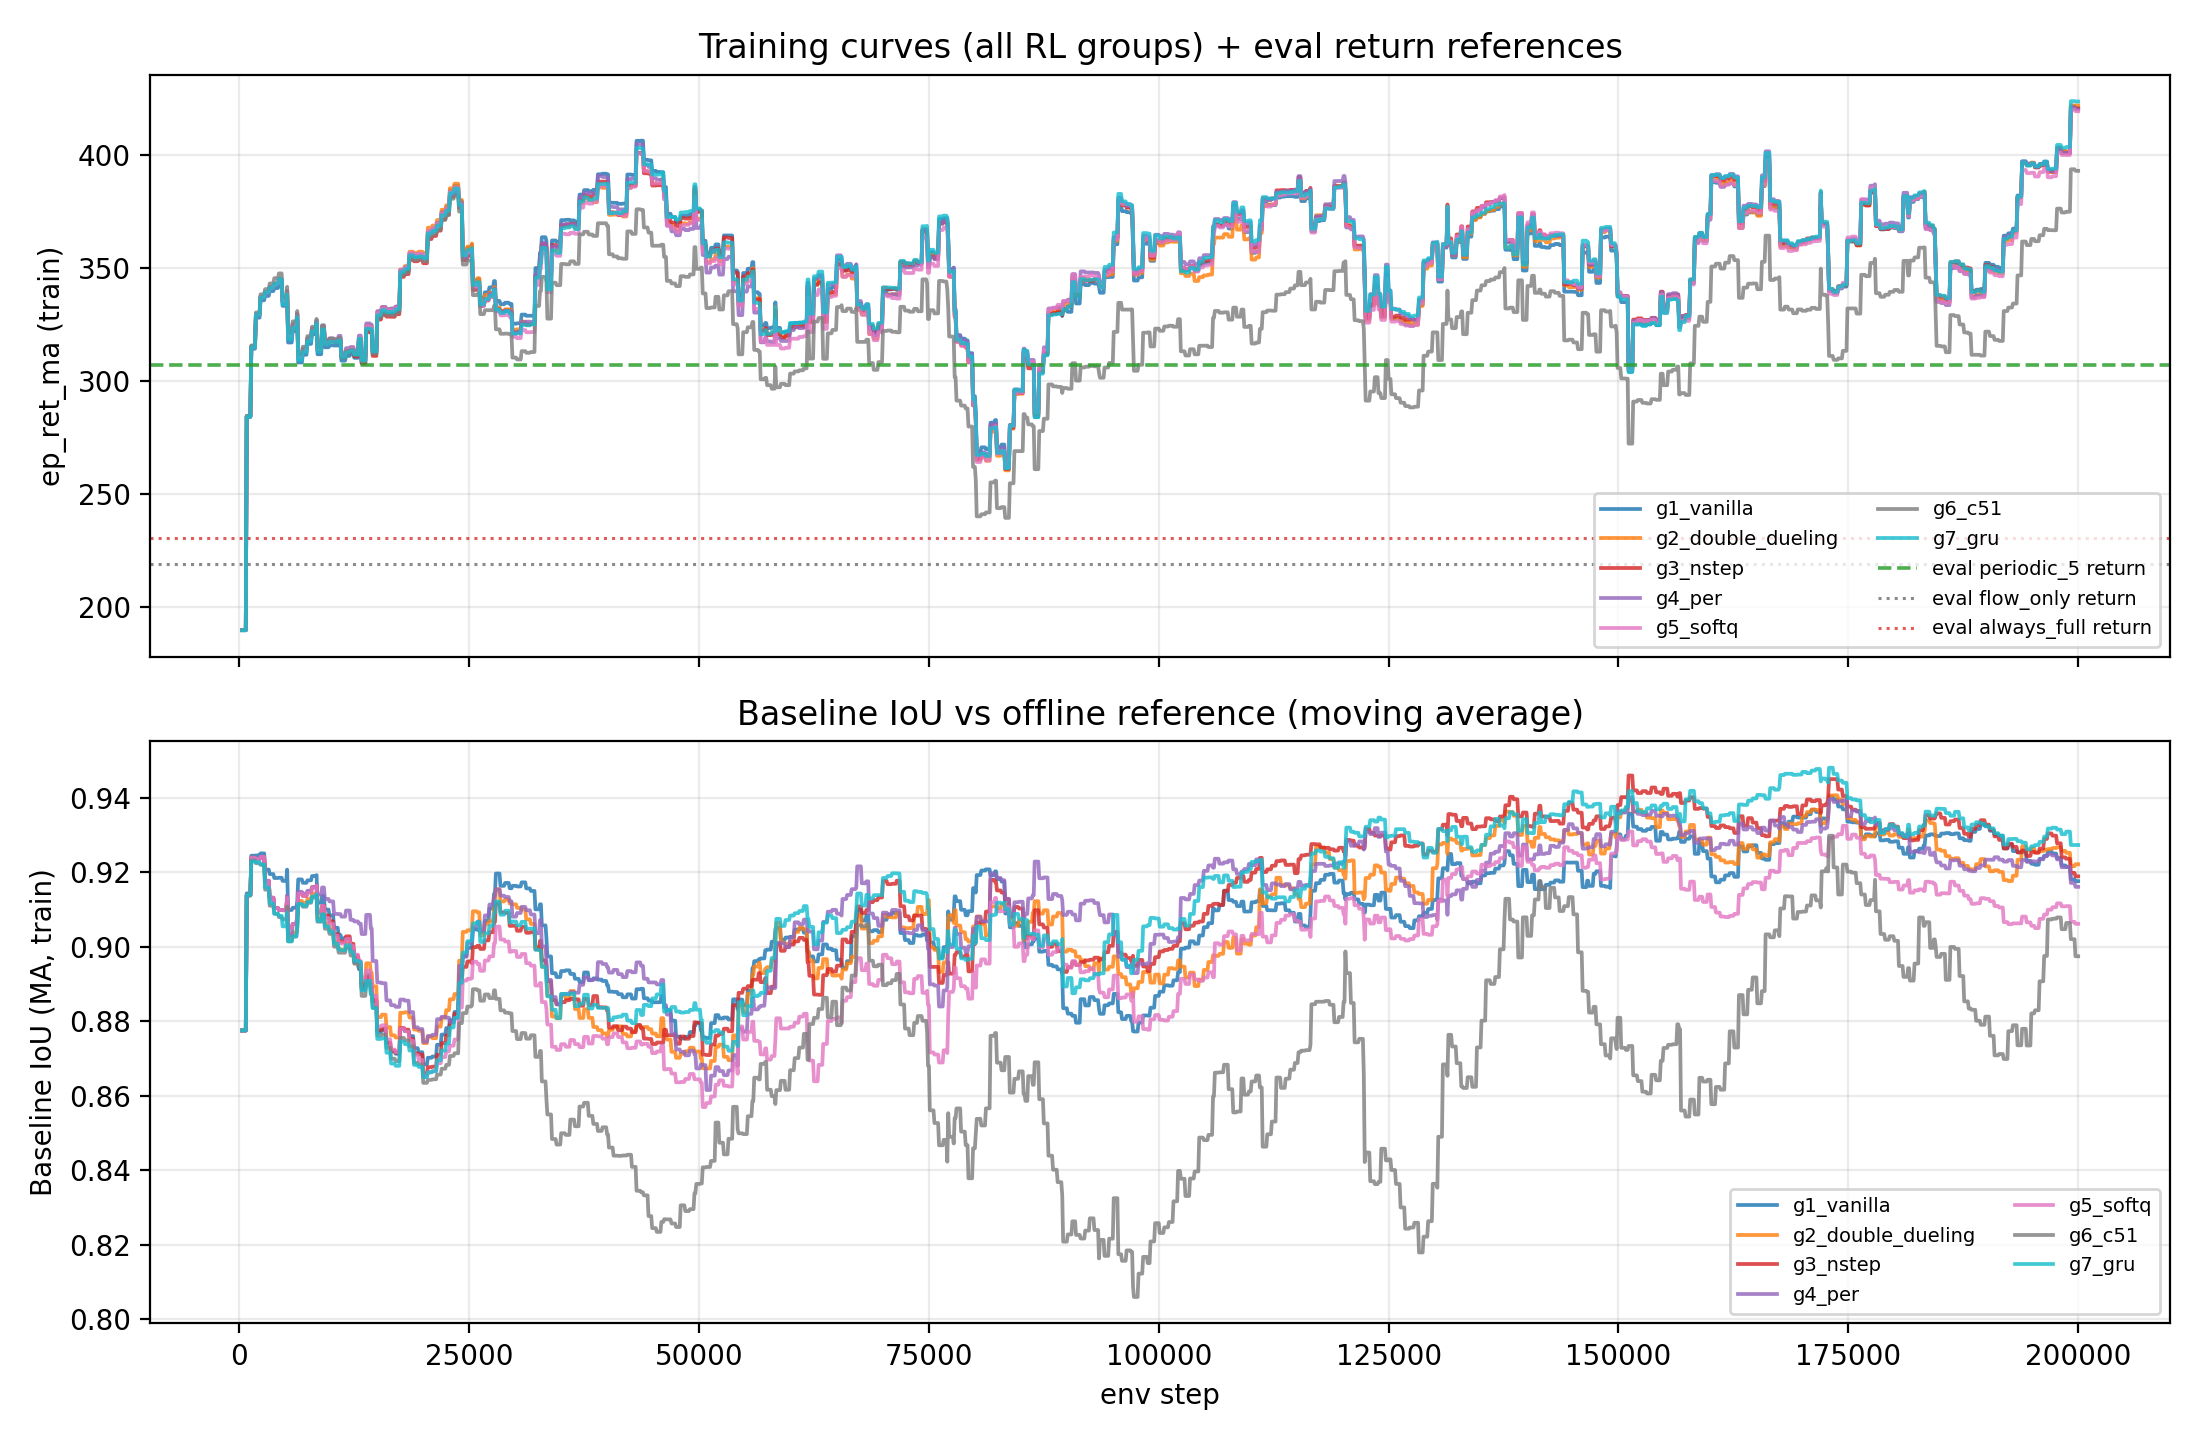
\includegraphics[width=0.92\linewidth]{plots/01_learning_curves_overview.png}
\caption{Training-dynamics overview for RL groups (50k-step budget): per-group curves aggregated from training logs (e.g., moving averages of return, reference IoU when logged, loss/TD diagnostics). Not identical to greedy eval in Table~\ref{tab:summary_full}.}
\label{fig:learning}
\end{figure}%
\noindent\textbf{Analysis for Fig.~\ref{fig:learning}.}
This figure summarizes \emph{training-time} dynamics (one curve per RL group under the shared budget in Section~\ref{sec:method}), not the held-out greedy evaluation in Table~\ref{tab:summary_full}. Read it as a sanity check on optimization: curves should be finite, without exploding loss scales or repeated NaNs across steps. Smooth late-stage plateaus often correlate with stable value targets. Because the reward couples quality and cost, TD learning can be sensitive to reward-scale drift: by default, trainers update $\lambda_{\mathrm{cost}}$ at episode boundaries unless \texttt{fixed\_lambda} is enabled (Table~\ref{tab:hparams}), whereas headline evaluation fixes $\lambda_{\mathrm{cost}}=0.35$.

Training stability is \emph{necessary} but not \emph{sufficient}: two groups can look equally ``flat'' while ending at different competence because backups, replay, and representation capacity change what the same data teaches~\cite{hessel2018rainbow}. In particular, methods that incorporate stronger target operators or distributional heads can converge slowly or to different local behaviors under small budgets. Finally, note the evaluation uses the saved \texttt{last} checkpoint in greedy mode; training curves therefore explain \textbf{how} a policy was produced, while bars and tables explain \textbf{how} it behaves on the logged eval suite.

\begin{figure}[H]
\centering
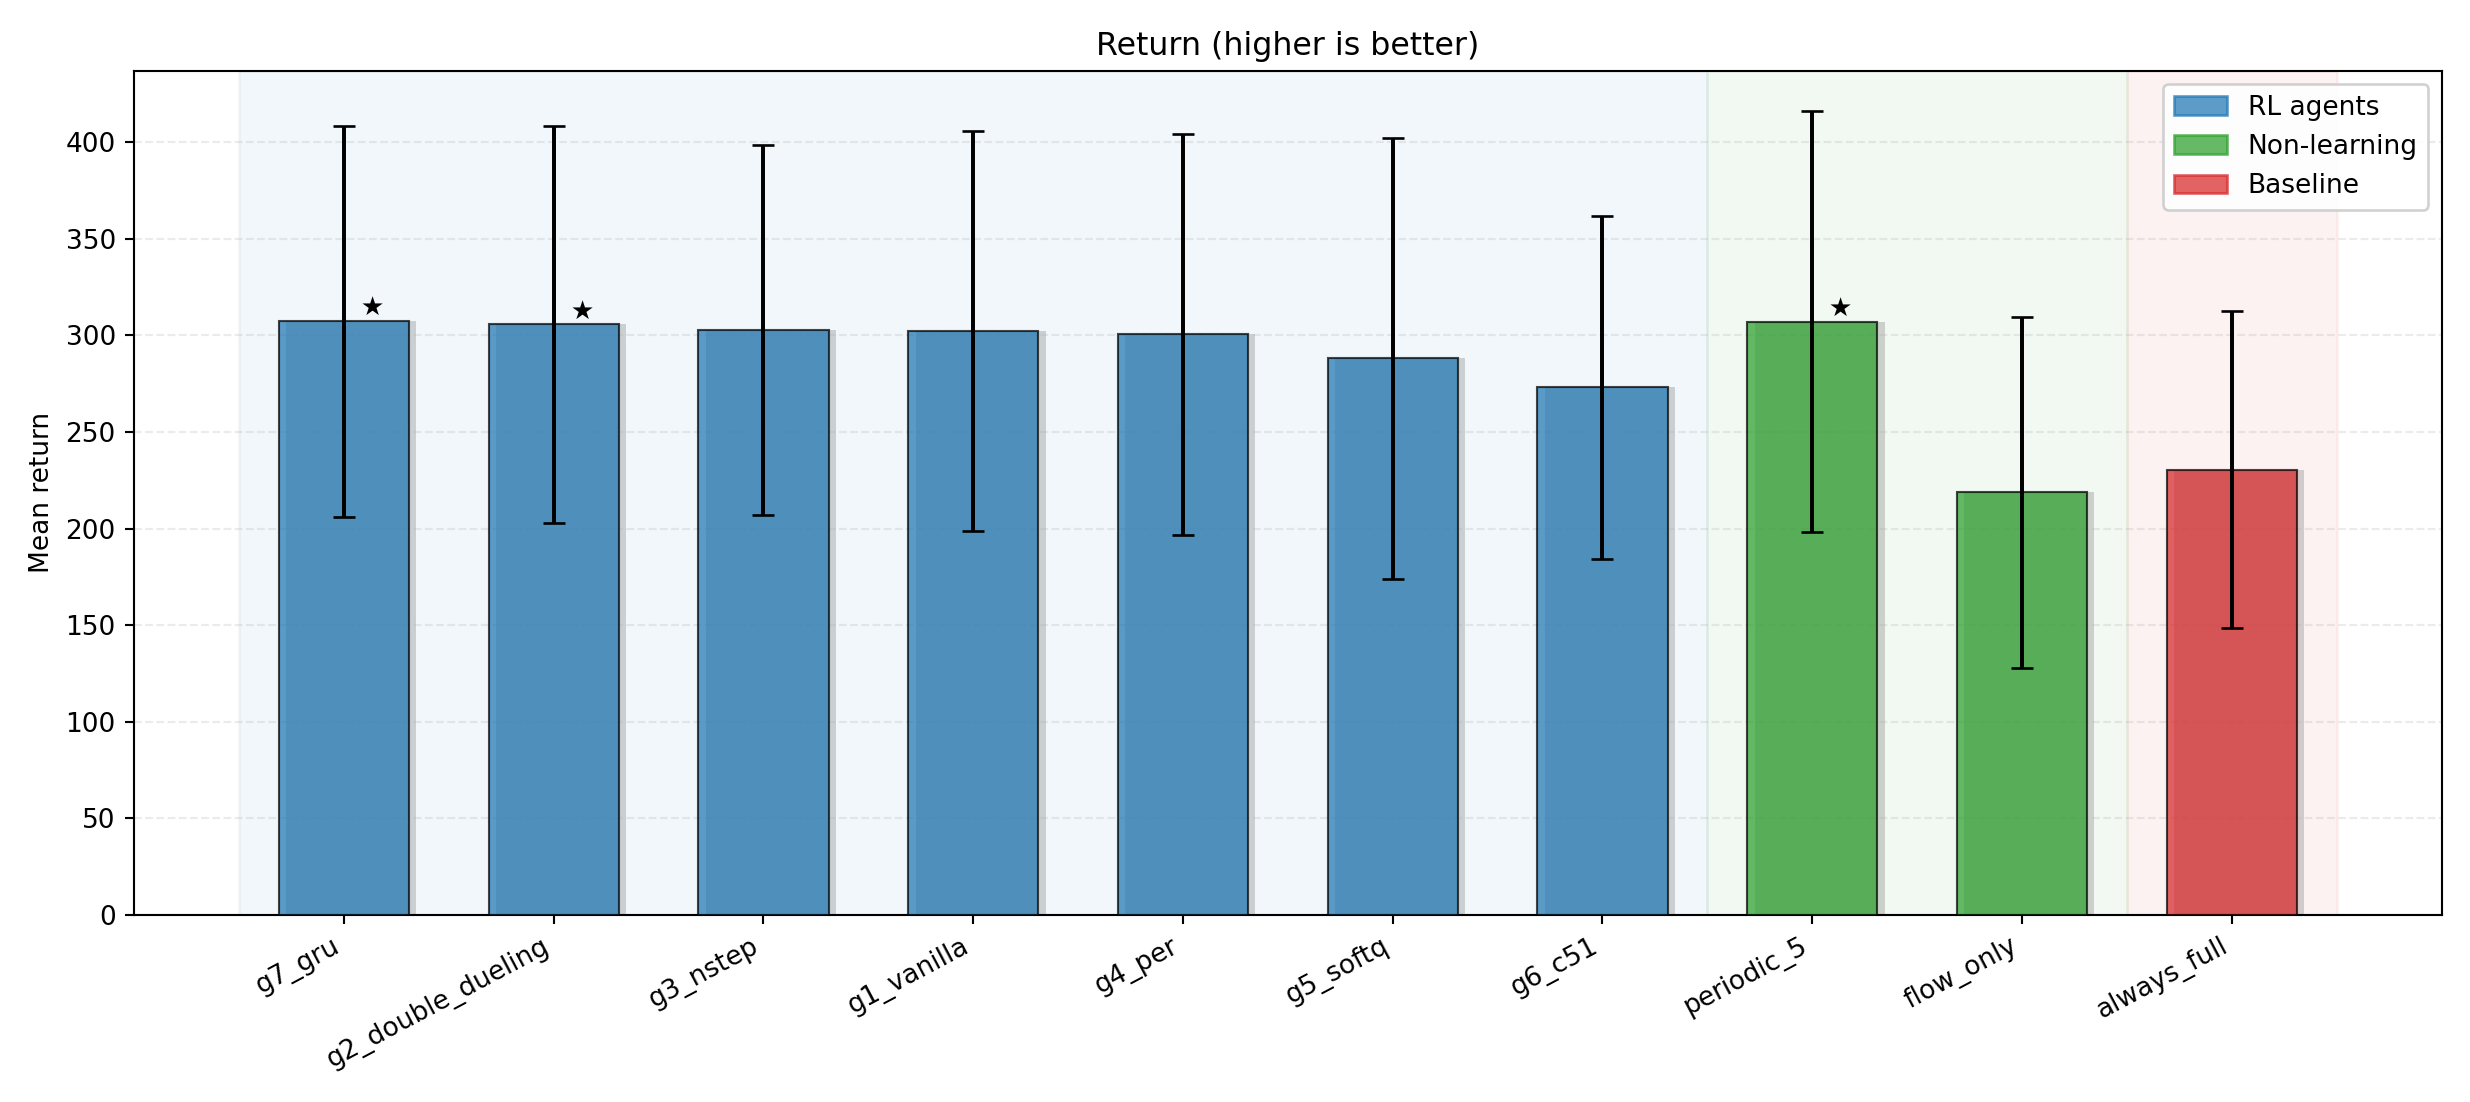
\includegraphics[width=0.96\linewidth]{plots/02_return_bar_comparison.png}
\caption{Mean episodic return with dispersion across three eval episodes (higher is better). RL bars sorted by mean; colors group RL vs.\ non-learning vs.\ always-on baseline.}
\label{fig:return_bar}
\end{figure}%
\noindent\textbf{Analysis for Fig.~\ref{fig:return_bar}.}
Each bar is the mean episodic return with error bars reflecting dispersion across the three evaluation episodes (same raw file as Table~\ref{tab:summary_full}). Policies are grouped visually by type (RL agents, non-learning rules, and the always-on baseline), and RL bars are sorted by return so the figure doubles as a ranked scoreboard.

Return aggregates per-step rewards (Eq.~\eqref{eq:reward}; $\alpha{=}1$ and fixed $\lambda_{\mathrm{cost}}$ at evaluation), so a high bar indicates sustained reference IoU without paying excessive action costs. G7-GRU, Periodic-5, and G2-DDQ form a clear top tier in Table~\ref{tab:summary_full}, which matches the intuition that strong policies either correct often enough (without wasting full steps) or exploit a good schedule. Mid-tier methods (e.g., G5-SoftQ) suggest backup mismatch: optimization can finish, but the induced value targets may under-emphasize corrections needed after drift. Low-return extremes typically reflect either chronic under-correction (insufficient $q_t$) or inefficient spending on expensive actions that do not move $q_t$ enough to justify their $c(a_t)$.

\begin{figure}[H]
\centering
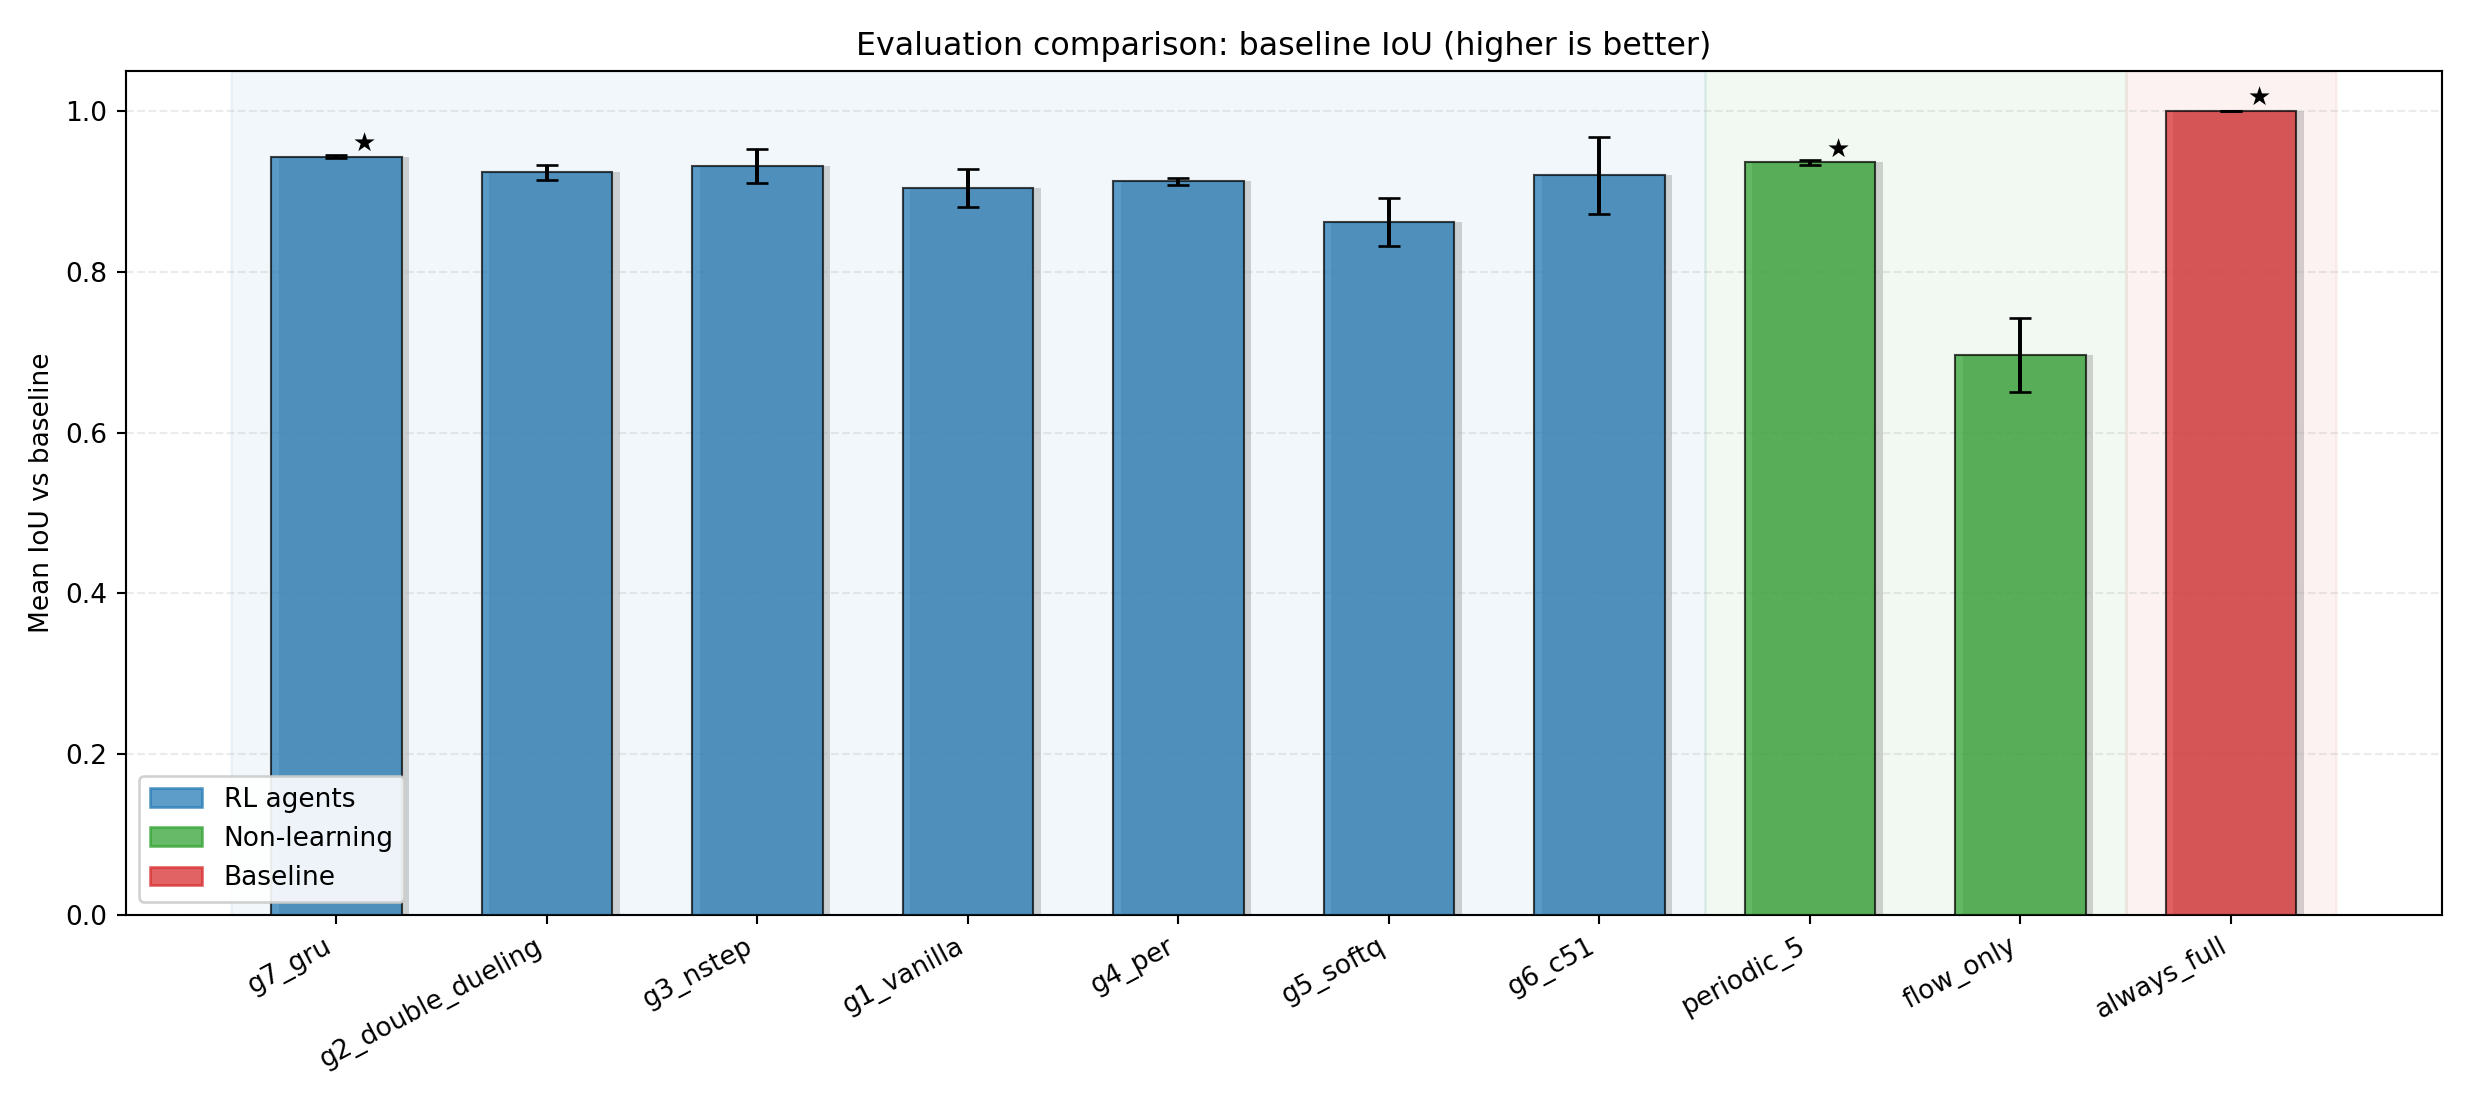
\includegraphics[width=0.96\linewidth]{plots/03_iou_bar_comparison.png}
\caption{Mean reference IoU (higher is better). Always-Full is the protocol's quality upper bound; other policies reveal the compute--quality trade-off.}
\label{fig:iou_bar}
\end{figure}%
\noindent\textbf{Analysis for Fig.~\ref{fig:iou_bar}.}
Mean IoU here is \emph{only} the alignment proxy $q_t$ averaged over time and episodes; it does not encode compute. Always-Full should sit at the ceiling because it invokes the strongest correction operator every step. The substantive comparison is therefore among policies that actually exercise the compute--quality trade-off.

G7-GRU and Periodic-5 reach the strongest IoU among those practical policies, which supports two points: (i) periodic full inference is a strong structural prior when motion is predictable, and (ii) a recurrent value function can recover similar alignment while adapting to local difficulty rather than committing to a fixed cadence. Conversely, Flow-Only illustrates failure under always-cheap updates: IoU collapses because drift accumulates faster than the lightweight operator can repair. Intermediate policies (e.g., G5-SoftQ) show that high IoU is not automatic even when return is ``reasonable,'' underscoring that IoU and return are coupled but not identical under partial observability and action costs.

\begin{figure}[H]
\centering
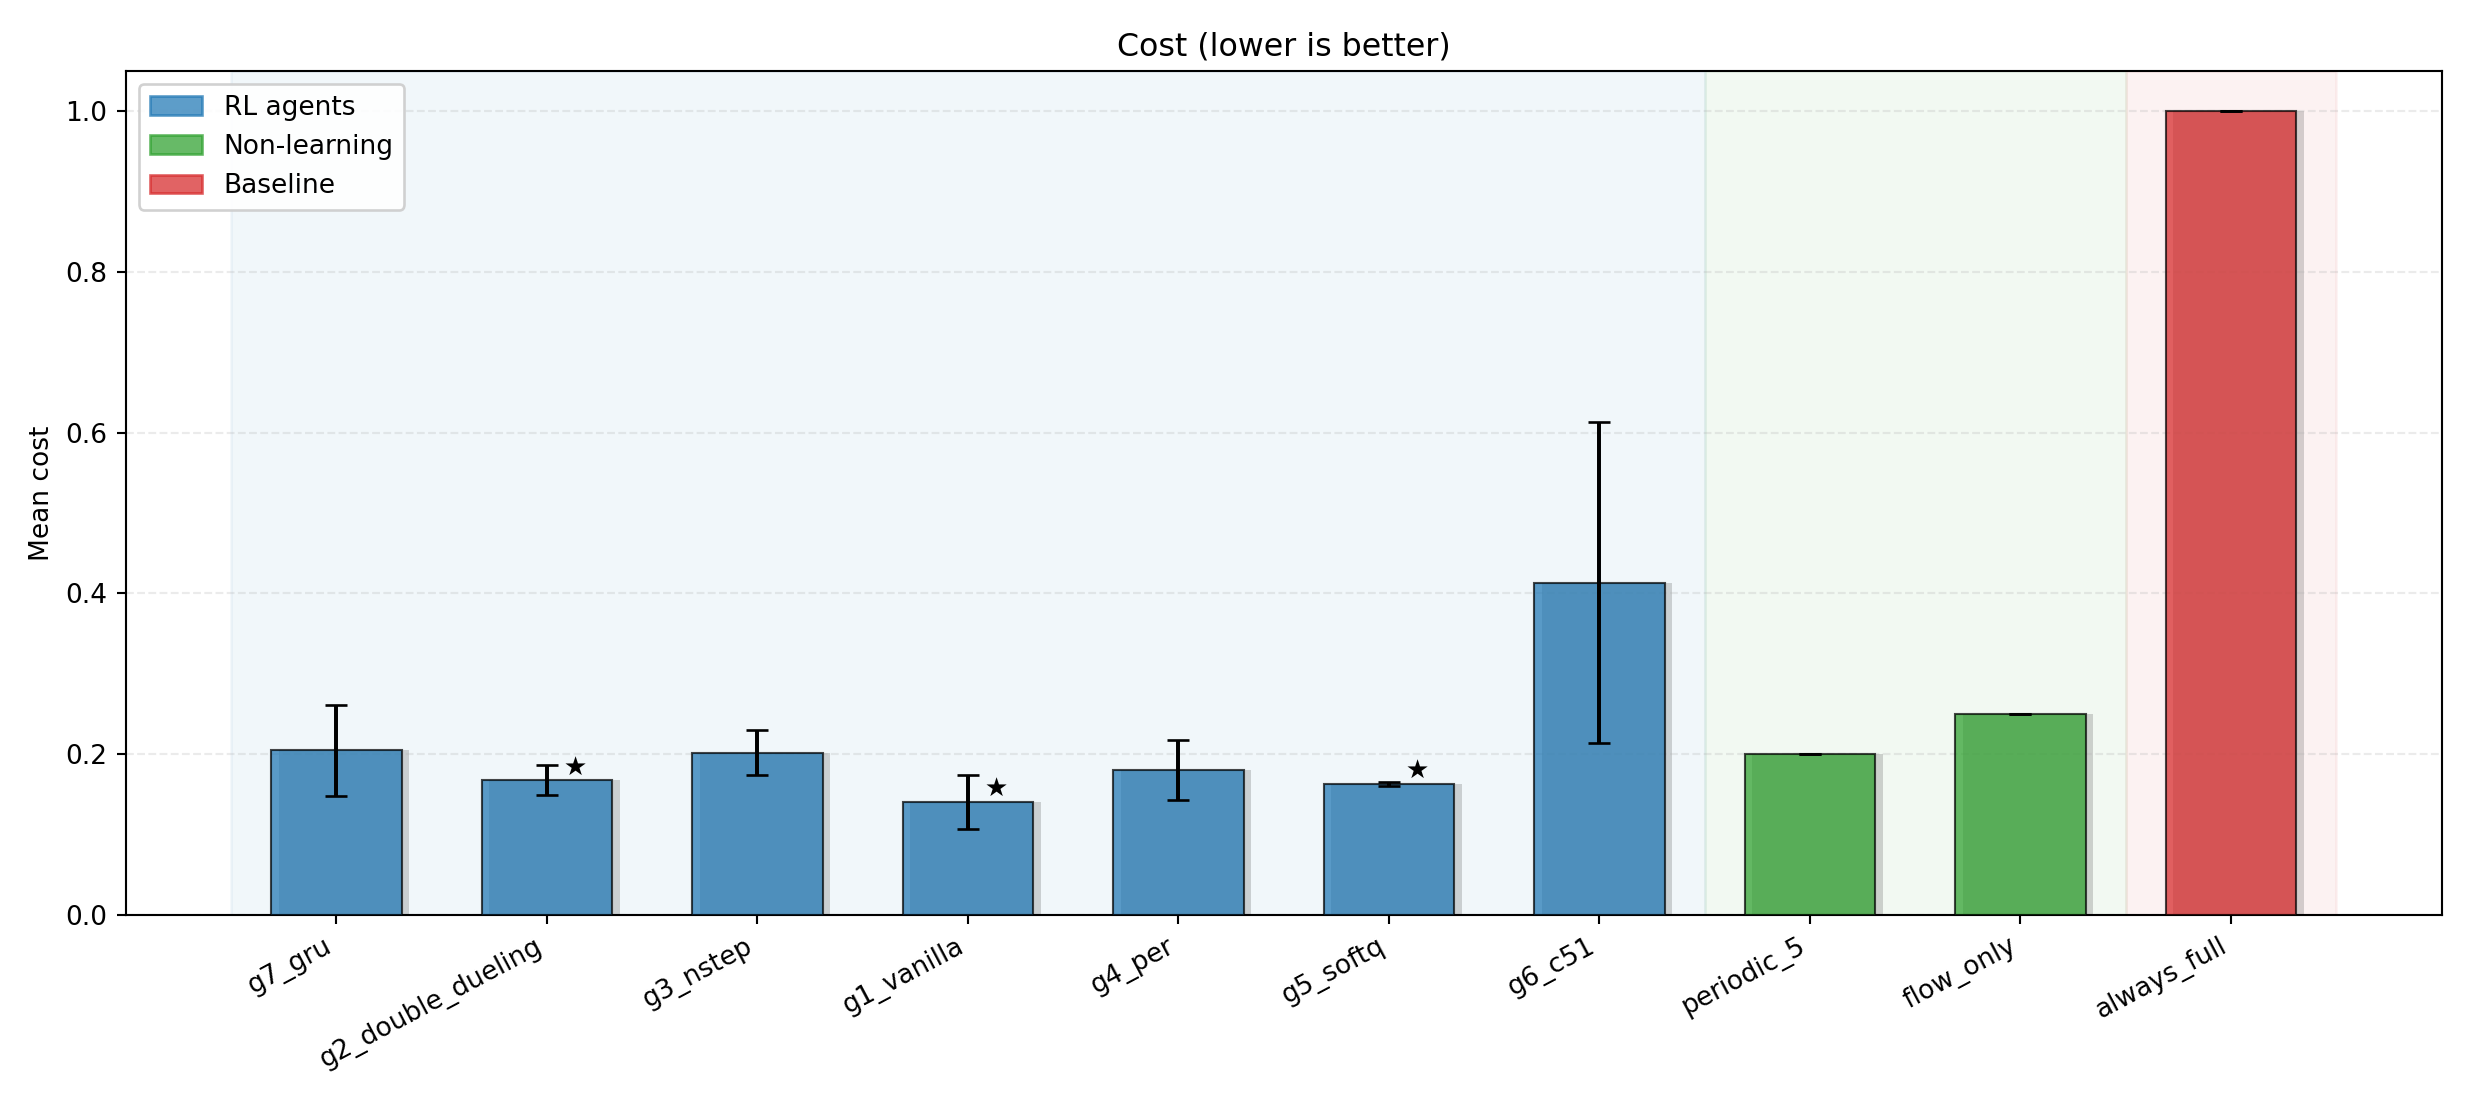
\includegraphics[width=0.96\linewidth]{plots/04_cost_bar_comparison.png}
\caption{Mean per-step action cost (lower is better). Always-Full attains maximal cost by construction.}
\label{fig:cost_bar}
\end{figure}%
\noindent\textbf{Analysis for Fig.~\ref{fig:cost_bar}.}
Mean cost reports $\mathbb{E}[c(a_t)]$ under each policy, using the same cost model as training and evaluation (Section~\ref{sec:problem}). Always-Full defines the upper bound by construction. Learned policies should populate the interior: the interesting question is whether reduced cost comes from \emph{intelligent} skipping of full steps or from \emph{under}-invocation that harms IoU.

Reading this figure next to Fig.~\ref{fig:iou_bar} separates those cases. G1-Vanilla achieves very low average cost in Table~\ref{tab:summary_full}, which is attractive only because its IoU remains acceptable for the task; if cost were low \emph{and} IoU collapsed, that would indicate pathological under-sampling of \texttt{FULL\_DETECT}. G6-C51 is the opposite diagnostic: it pays high average cost while still trailing G7-GRU on IoU, suggesting that ``spend more'' did not translate into proportionally better reference alignment under this checkpoint and budget---a concrete example of why cost must never be read without quality context.

\begin{figure}[H]
\centering
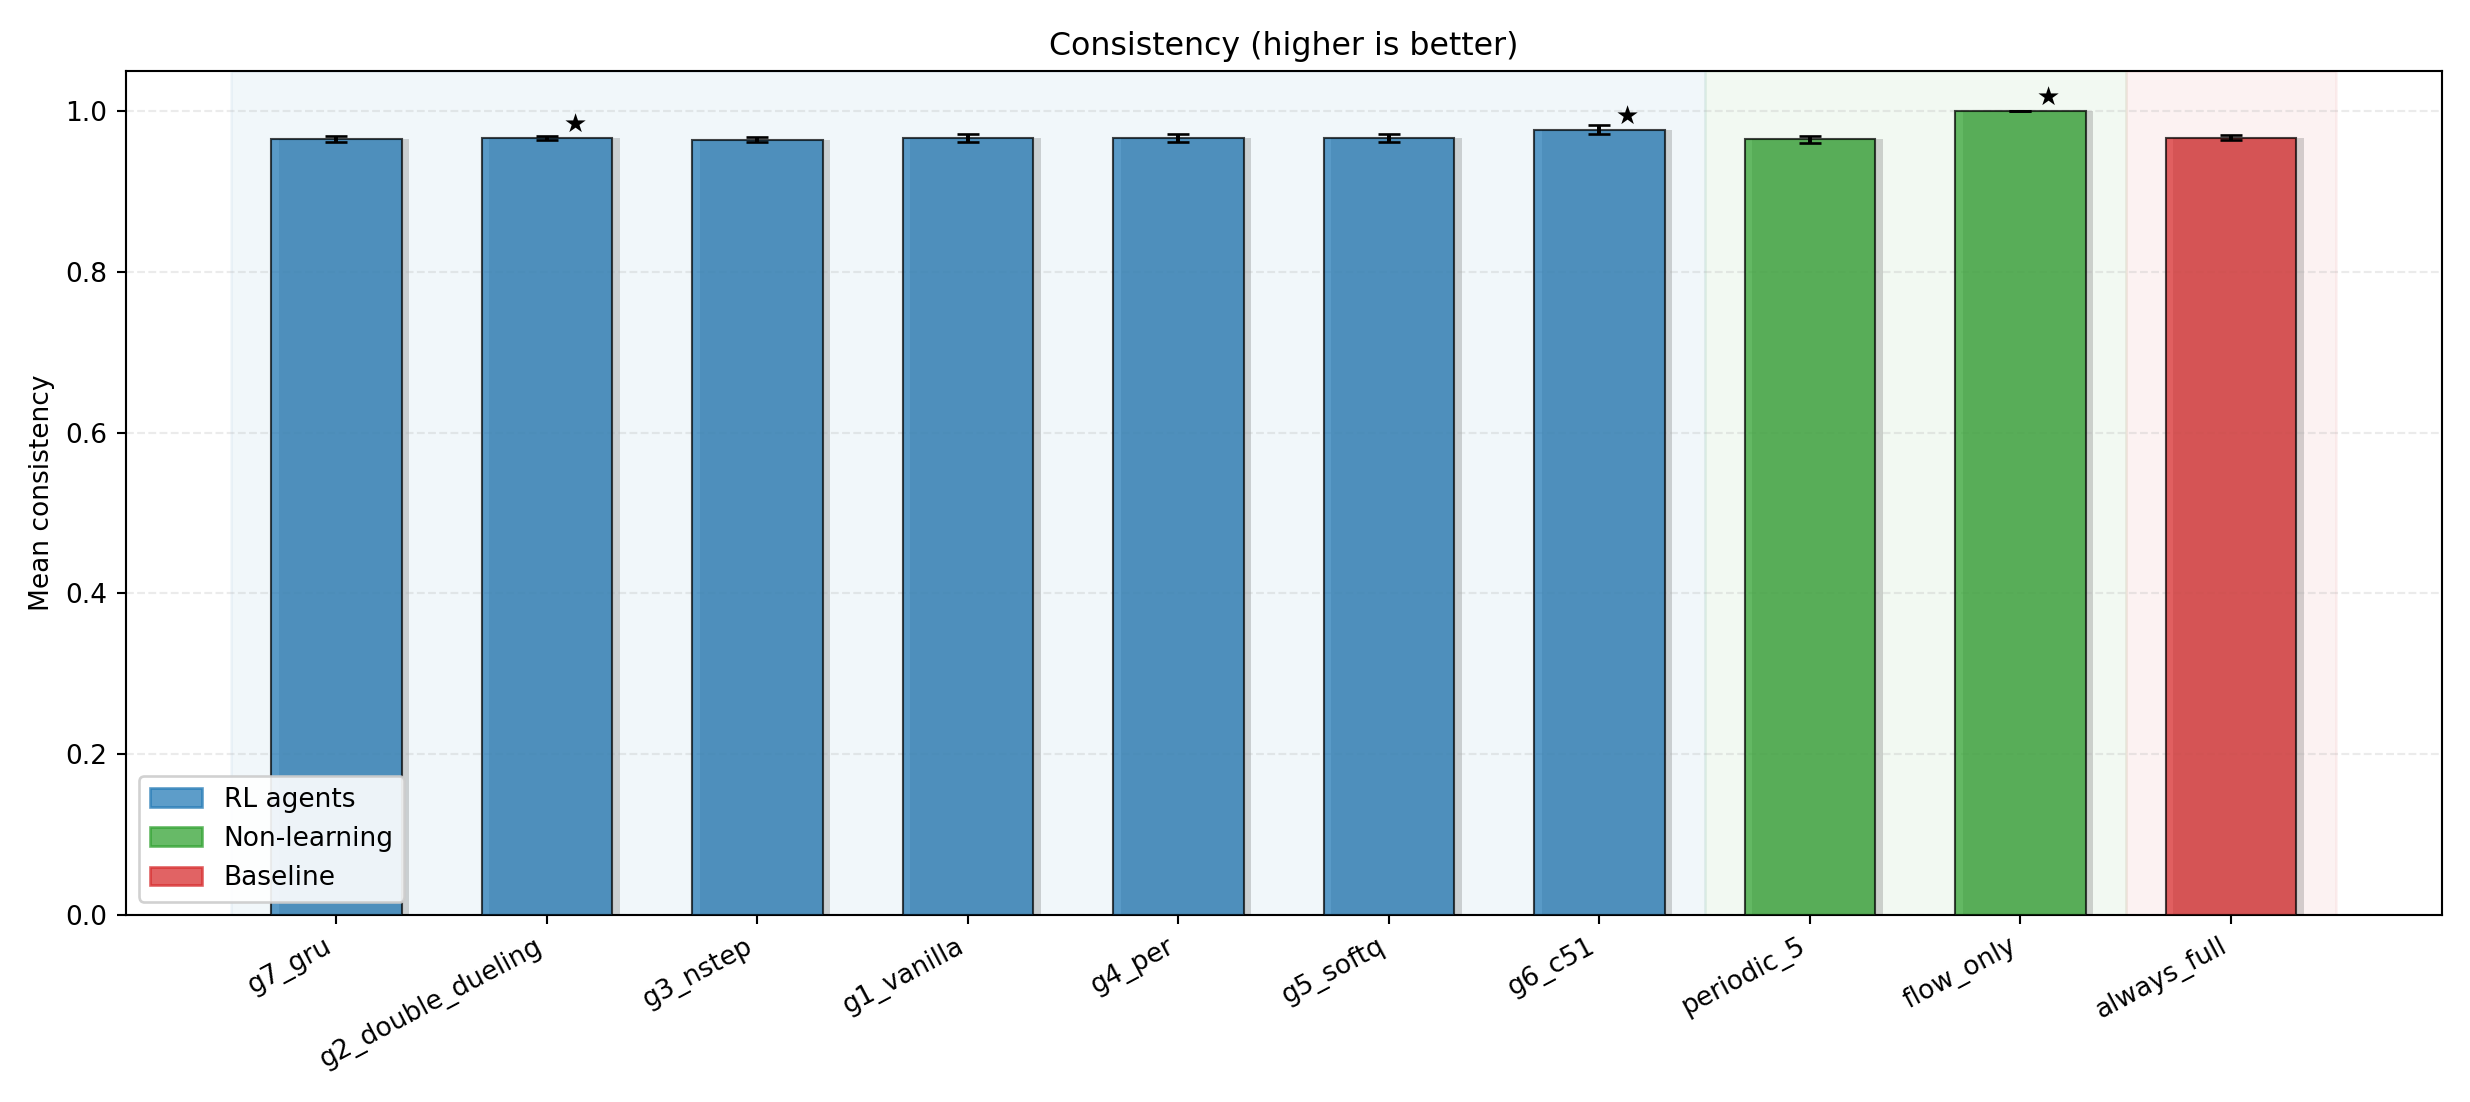
\includegraphics[width=0.96\linewidth]{plots/05_consistency_bar_comparison.png}
\caption{Mean temporal-consistency proxy from logs (diagnostic smoothness; interpret alongside IoU, not as a substitute).}
\label{fig:consistency_bar}
\end{figure}%
\noindent\textbf{Analysis for Fig.~\ref{fig:consistency_bar}.}
Consistency measures temporal smoothness of the published track signal (higher means fewer frame-to-frame jumps \emph{relative to the metric definition used in logging}). It is a \emph{diagnostic}, not a surrogate for correctness: a policy can be perfectly smooth yet systematically offset from the reference, which Flow-Only illustrates when consistency is high but IoU is poor.

For deployment, interpret consistency as a \textbf{risk screen}: among policies with similar IoU, higher consistency may reduce downstream jitter (e.g., for any module consuming box streams). Among policies with dissimilar IoU, prefer IoU-first ranking. The leading RL and periodic policies typically show competitive consistency \emph{and} strong IoU, which is the desirable ``smooth and right'' regime; always-on full detection can be smooth yet expensive, so again this axis is not a substitute for Fig.~\ref{fig:cost_bar}.

\begin{figure}[H]
\centering
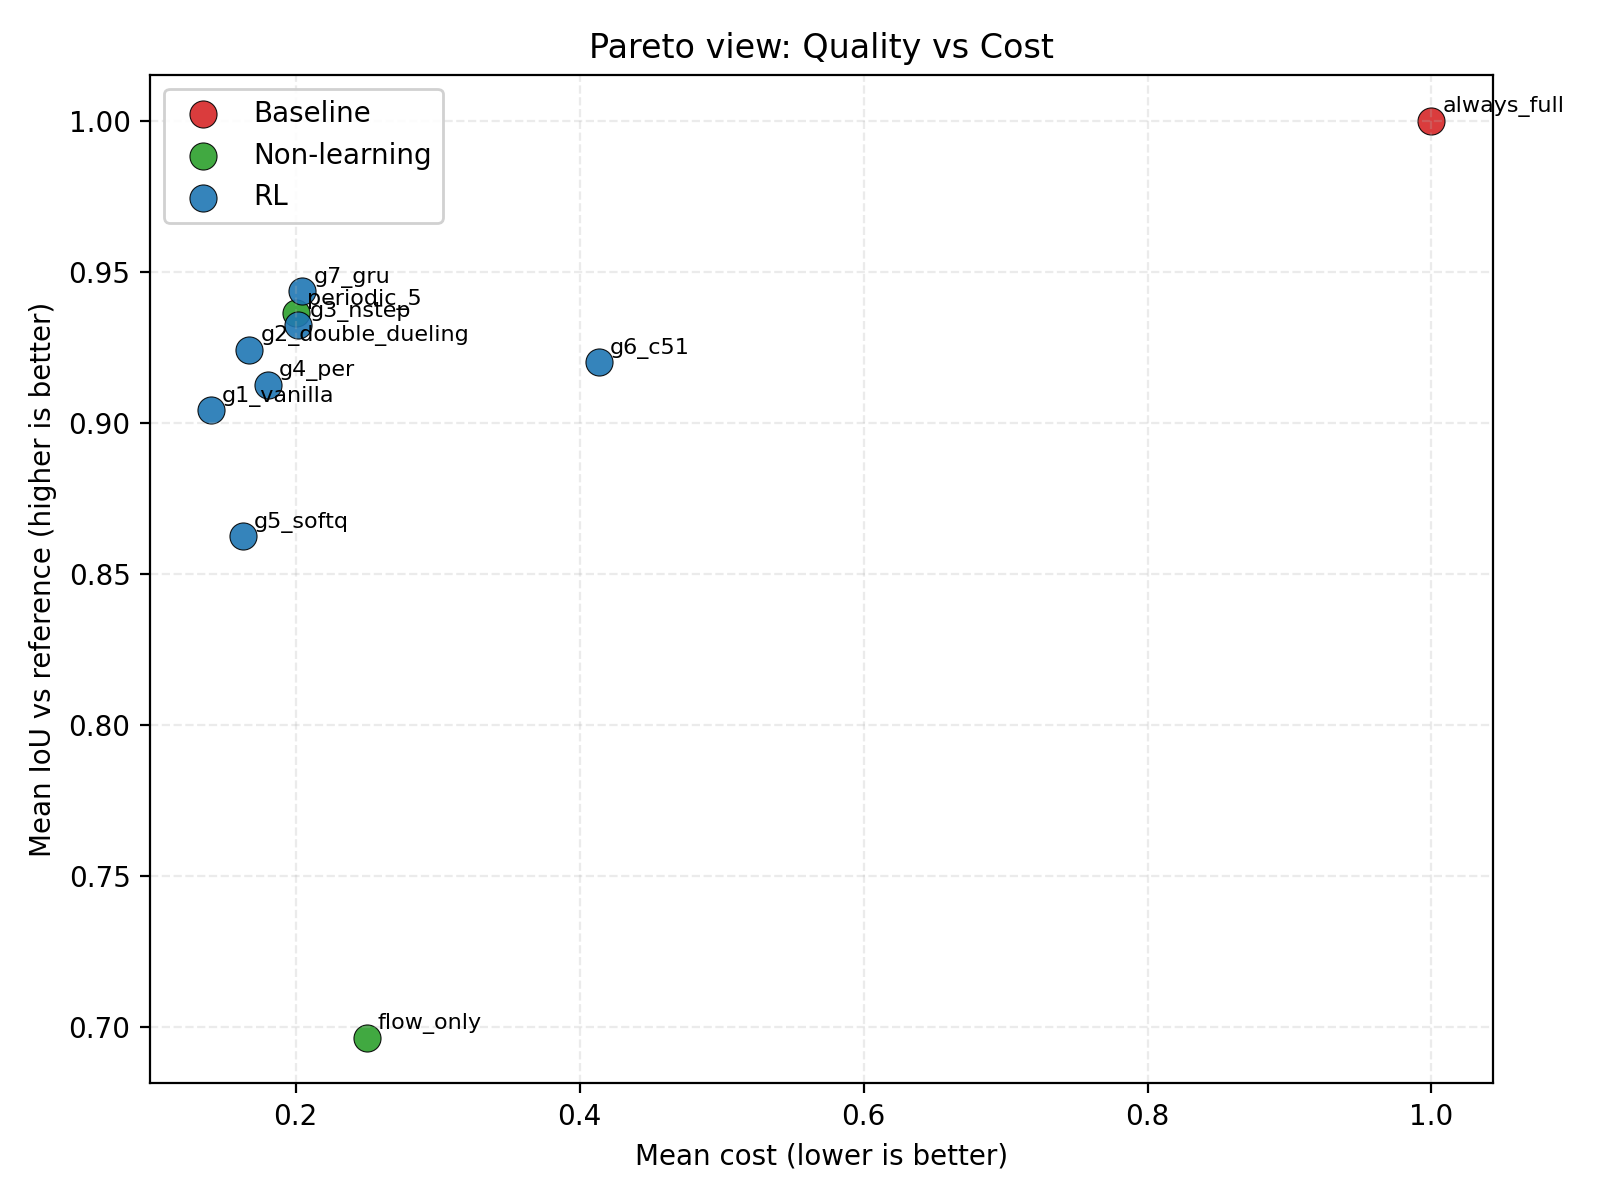
\includegraphics[width=0.96\linewidth]{plots/06_pareto_iou_vs_cost.png}
\caption{Quality--efficiency plane: mean reference IoU vs.\ mean action cost. Preferred region is upper-left (high IoU, low cost).}
\label{fig:pareto_iou_cost}
\end{figure}%
\noindent\textbf{Analysis for Fig.~\ref{fig:pareto_iou_cost}.}
Each point is one policy plotted in the natural deployment plane: vertical axis is reference IoU (quality), horizontal axis is mean action cost (lower is better). The ``ideal'' corner is therefore \textbf{upper-left}: strong alignment with cheap actions. Always-Full anchors the upper-\emph{right}: best IoU but worst cost, useful as a reference ruler rather than a competitor.

To read dominance informally, draw mental lines: if policy A is above and to the left of policy B, then A achieves better IoU at no higher cost (or strictly lower cost at no lower IoU) and is preferable under a monotone quality--cost preference. G7-GRU and Periodic-5 sit closest to the knee of the practical frontier in Table~\ref{tab:summary_full}, which is exactly the region an operator would shortlist. Points that lie low-left (low cost but collapsed IoU) are dominated for quality-sensitive deployments; points that lie mid-right spend heavily without reaching Always-Full IoU, signaling inefficiency rather than Pareto improvement.

\begin{figure}[H]
\centering
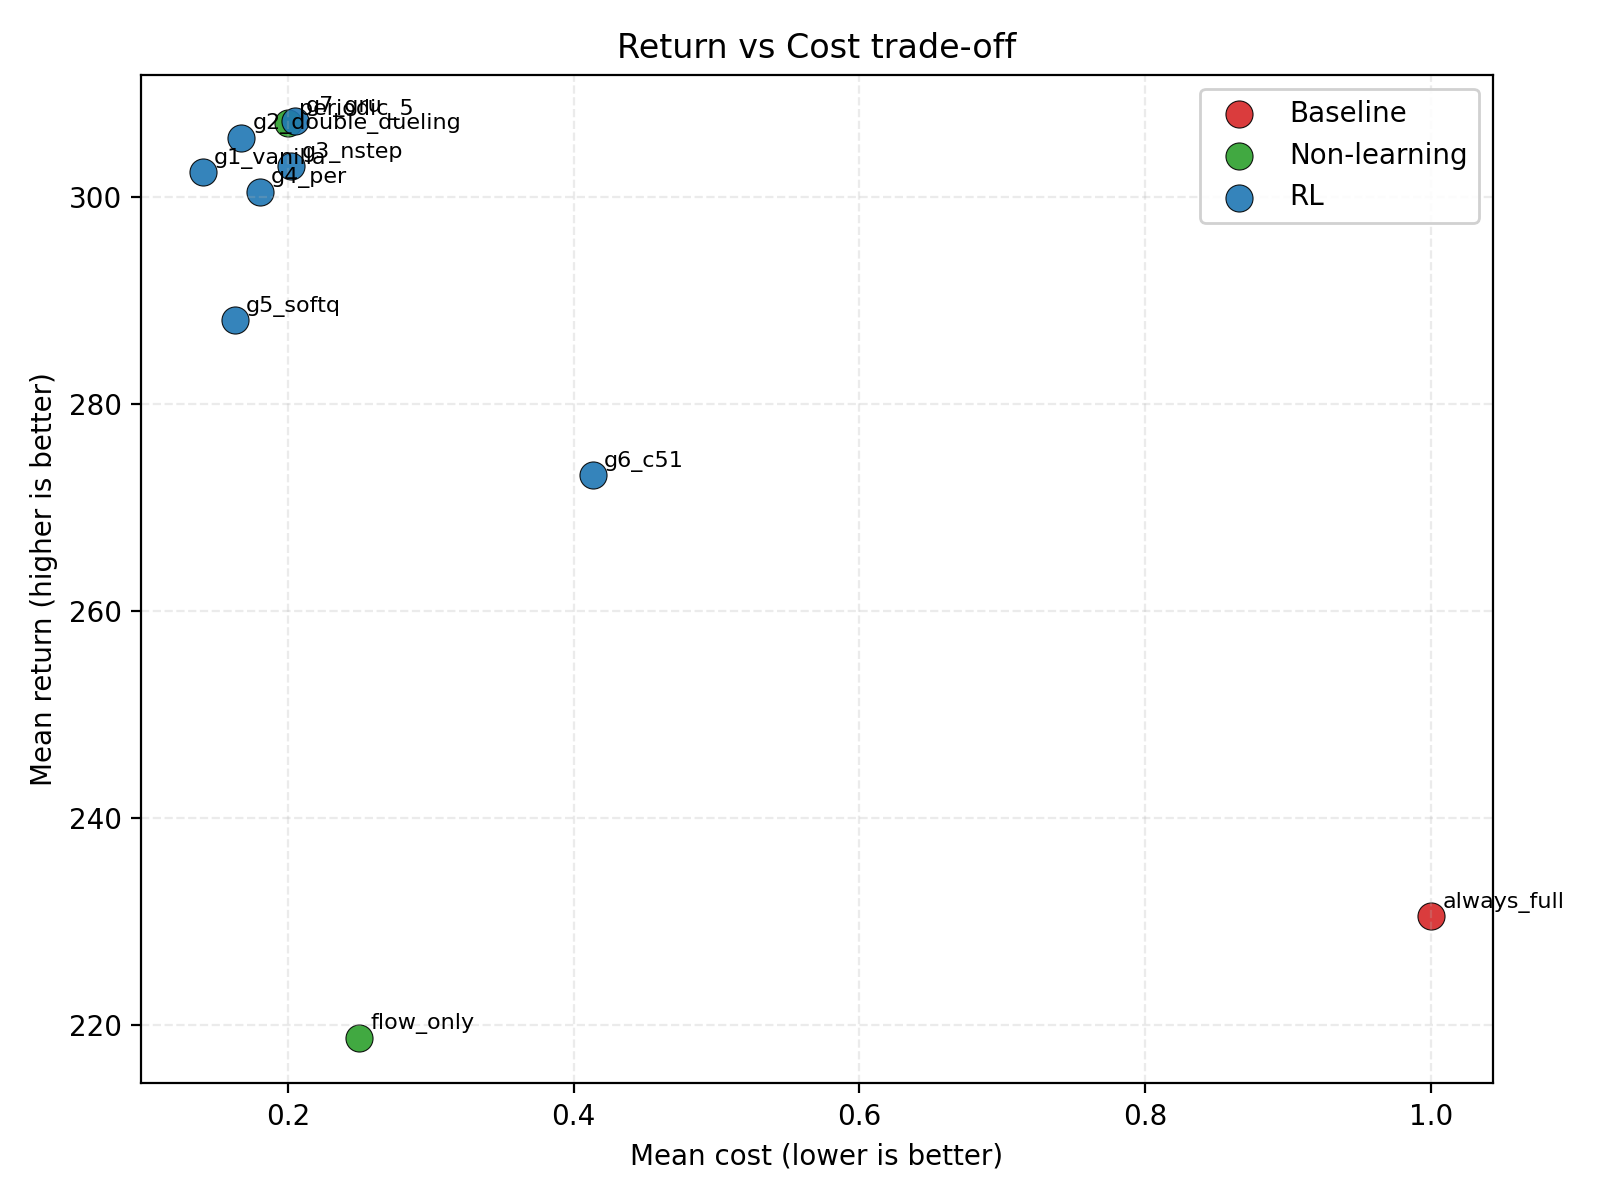
\includegraphics[width=0.96\linewidth]{plots/07_return_vs_cost_scatterplot.png}
\caption{Mean episodic return vs.\ mean action cost. Return integrates the logged reward (Eq.~\eqref{eq:reward}); eval fixes $\lambda_{\mathrm{cost}}{=}0.35$.}
\label{fig:return_cost}
\end{figure}%
\noindent\textbf{Analysis for Fig.~\ref{fig:return_cost}.}
This scatter replots the same policies in the plane of \emph{optimization objective} (return, which folds $q_t$ and $c(a_t)$ under Eq.~\eqref{eq:reward}) versus \emph{operational cost}. Training uses the same reward shape but may reschedule $\lambda_{\mathrm{cost}}$ across episodes (Table~\ref{tab:hparams}), whereas this panel uses evaluation means at fixed $\lambda_{\mathrm{cost}}{=}0.35$; exploration and partial observability still separate trained intent from logged eval points.

Policies in the upper-left (high return, low cost) are internally consistent: they earn high cumulative reward without paying maximal action prices. Policies below the cloud on return at similar cost are misaligned with the stated objective: they spend compute but do not translate it into reward, often because backups or heads mis-estimate the long-run value of occasional \texttt{FULL\_DETECT}. Policies far to the right with middling return resemble ``paying for insurance you do not use''---high-frequency corrections that do not move IoU enough to justify their penalty. Reading this figure together with Fig.~\ref{fig:pareto_iou_cost} checks whether a high return is earned via genuine quality gains (IoU) or via metric artifacts.

\begin{figure}[H]
\centering
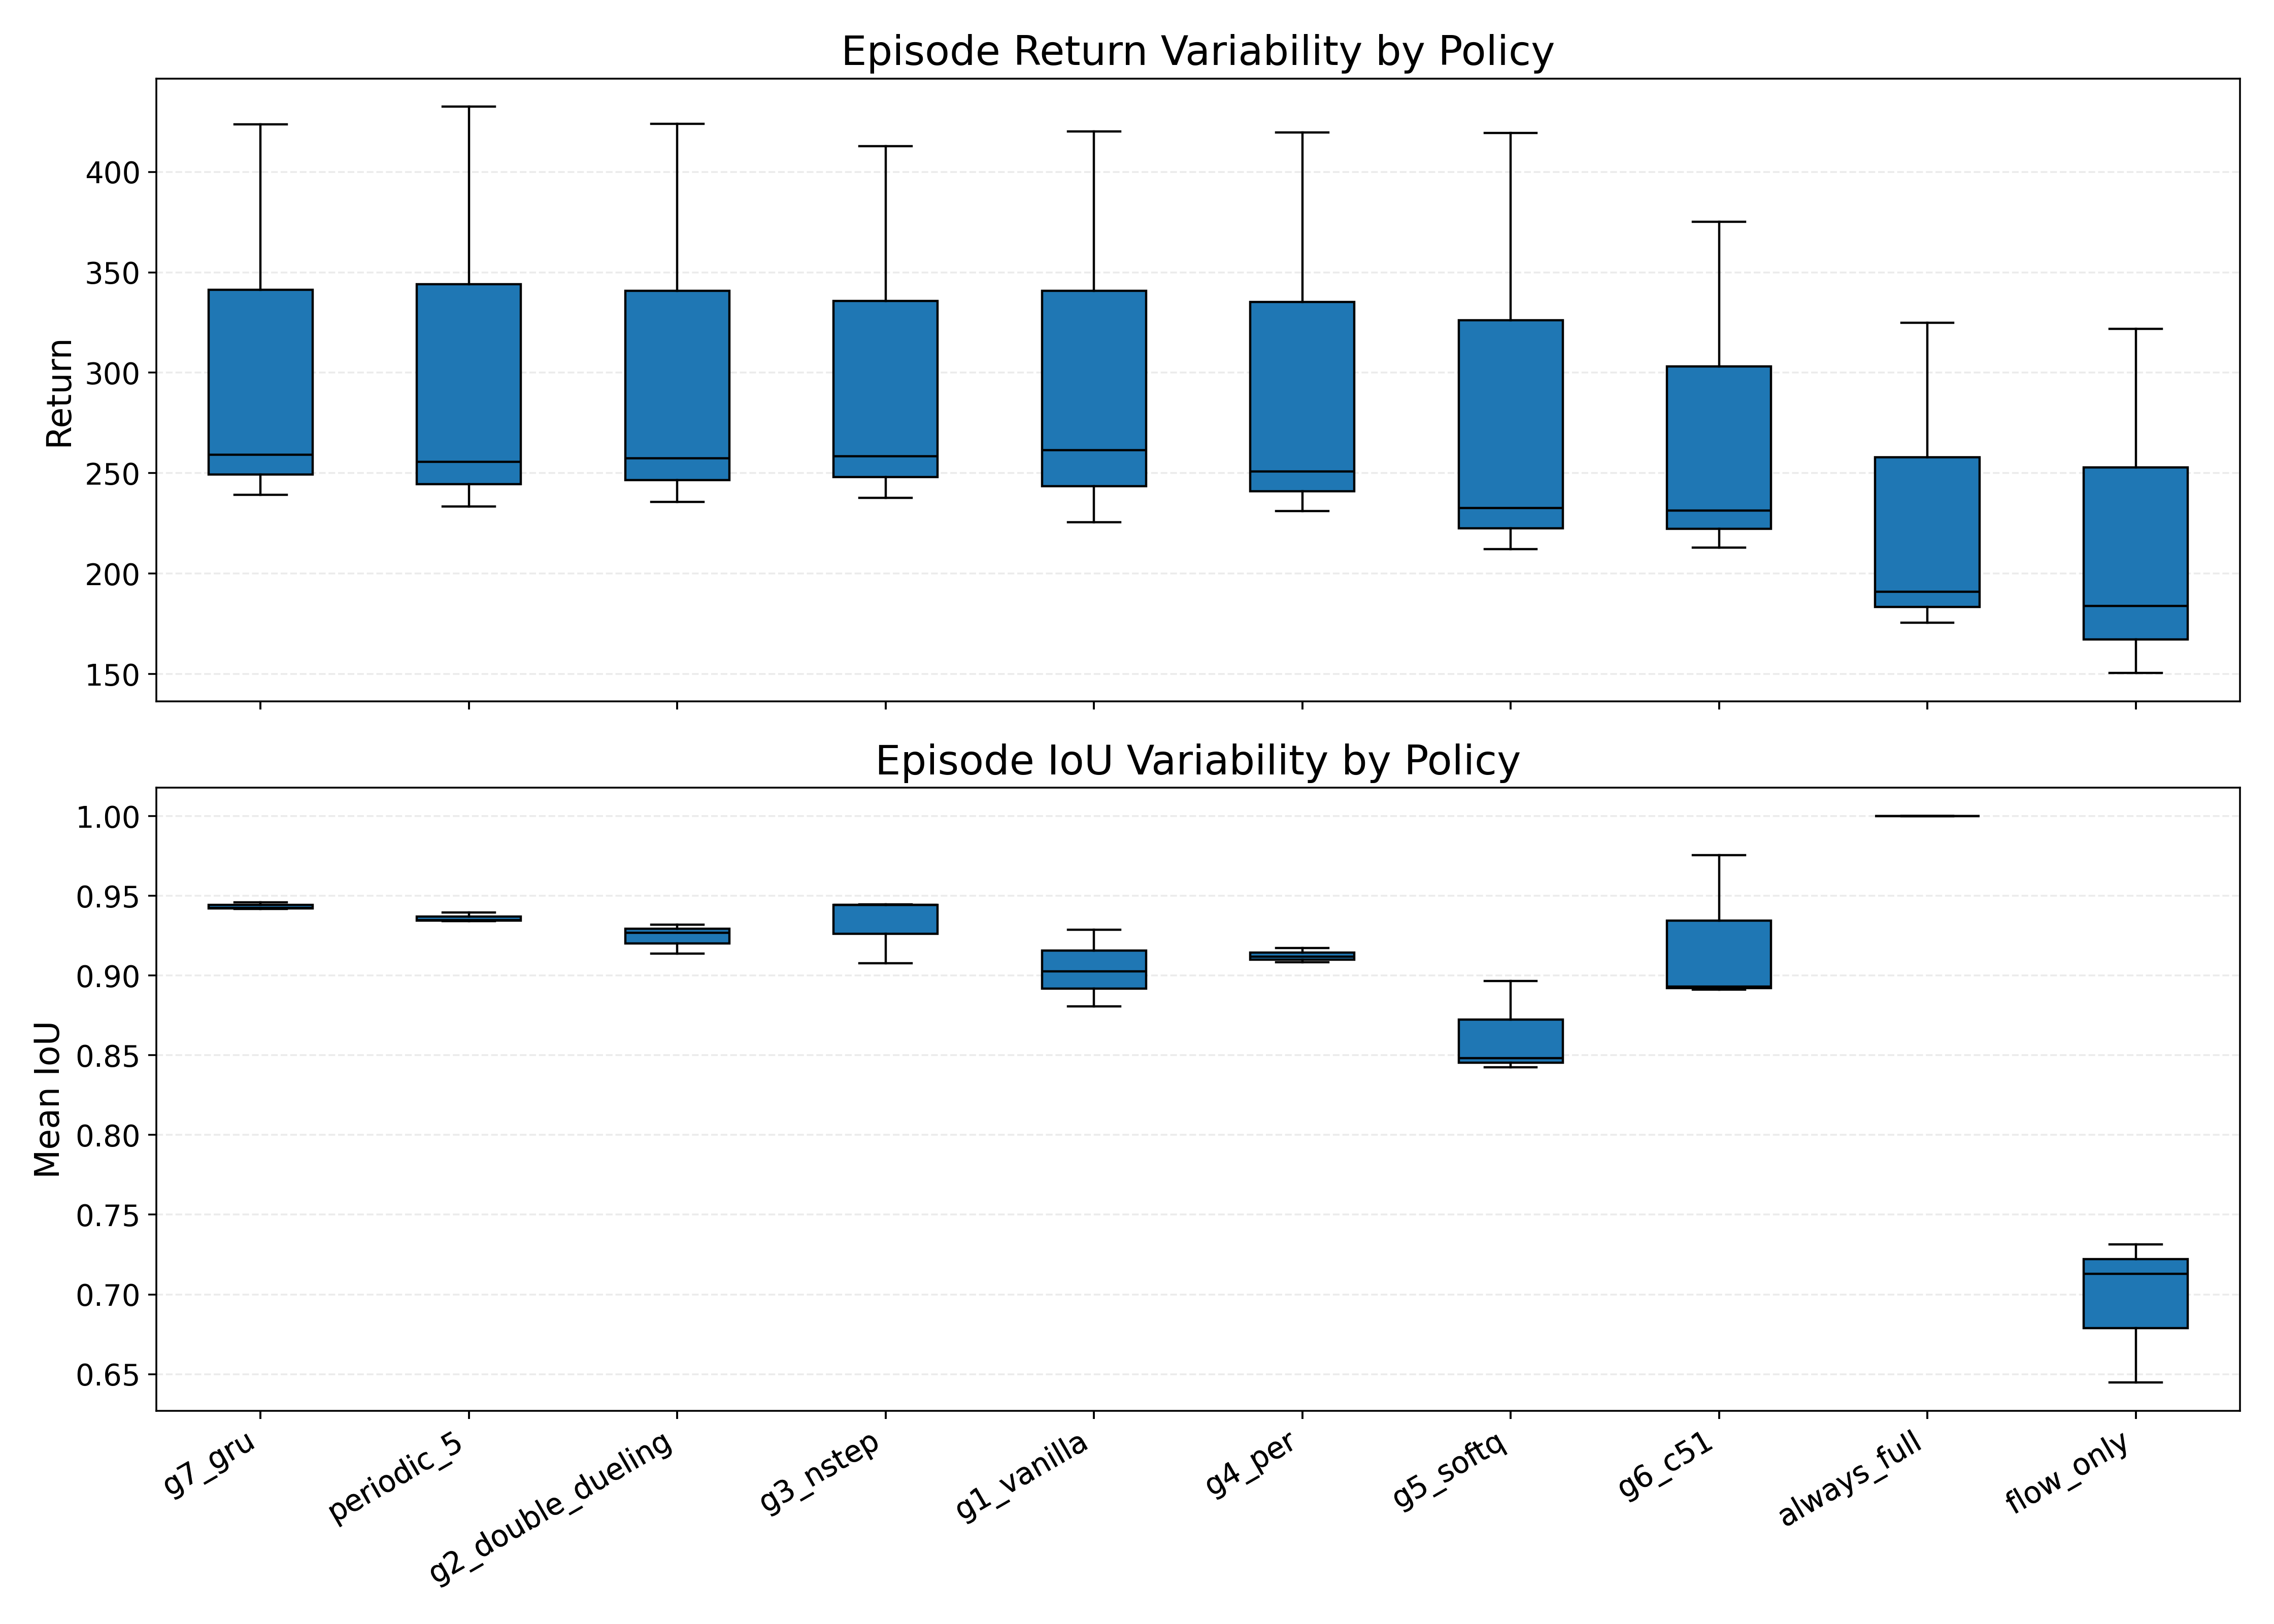
\includegraphics[width=0.92\linewidth]{plots/08_episode_variability_boxplot.png}
\caption{Episode-level return and reference IoU with three episodes per policy: read medians, spreads, and tails jointly with Table~\ref{tab:ci}.}
\label{fig:variability}
\end{figure}%
\noindent\textbf{Analysis for Fig.~\ref{fig:variability}.}
With only three episodes per policy, boxplots are sparse but still useful: the median line shows typical behavior, the box spans the middle episode spread, and whiskers/tails expose outlier-like behavior when one episode is much harder (e.g., a segment with fast motion or missed corrections).

Compare policies along \textbf{both} panels. A desirable policy has a high median return \emph{and} a tight IoU band near its mean; wide return swings mean the policy is gambling on rare high-reward segments, which is risky for deployment. Conversely, a narrow return box with poor IoU median means consistently bad alignment, not occasional bad luck. Top-tier policies should show competitive medians without extreme IoU tails; if a method shows acceptable mean IoU in Fig.~\ref{fig:iou_bar} but a heavy low tail here, that method may violate hard quality floors in a fraction of runs. This figure therefore operationalizes Table~\ref{tab:ci}: wide boxes are the geometric counterpart of large CI half-widths.

\begin{figure}[H]
\centering
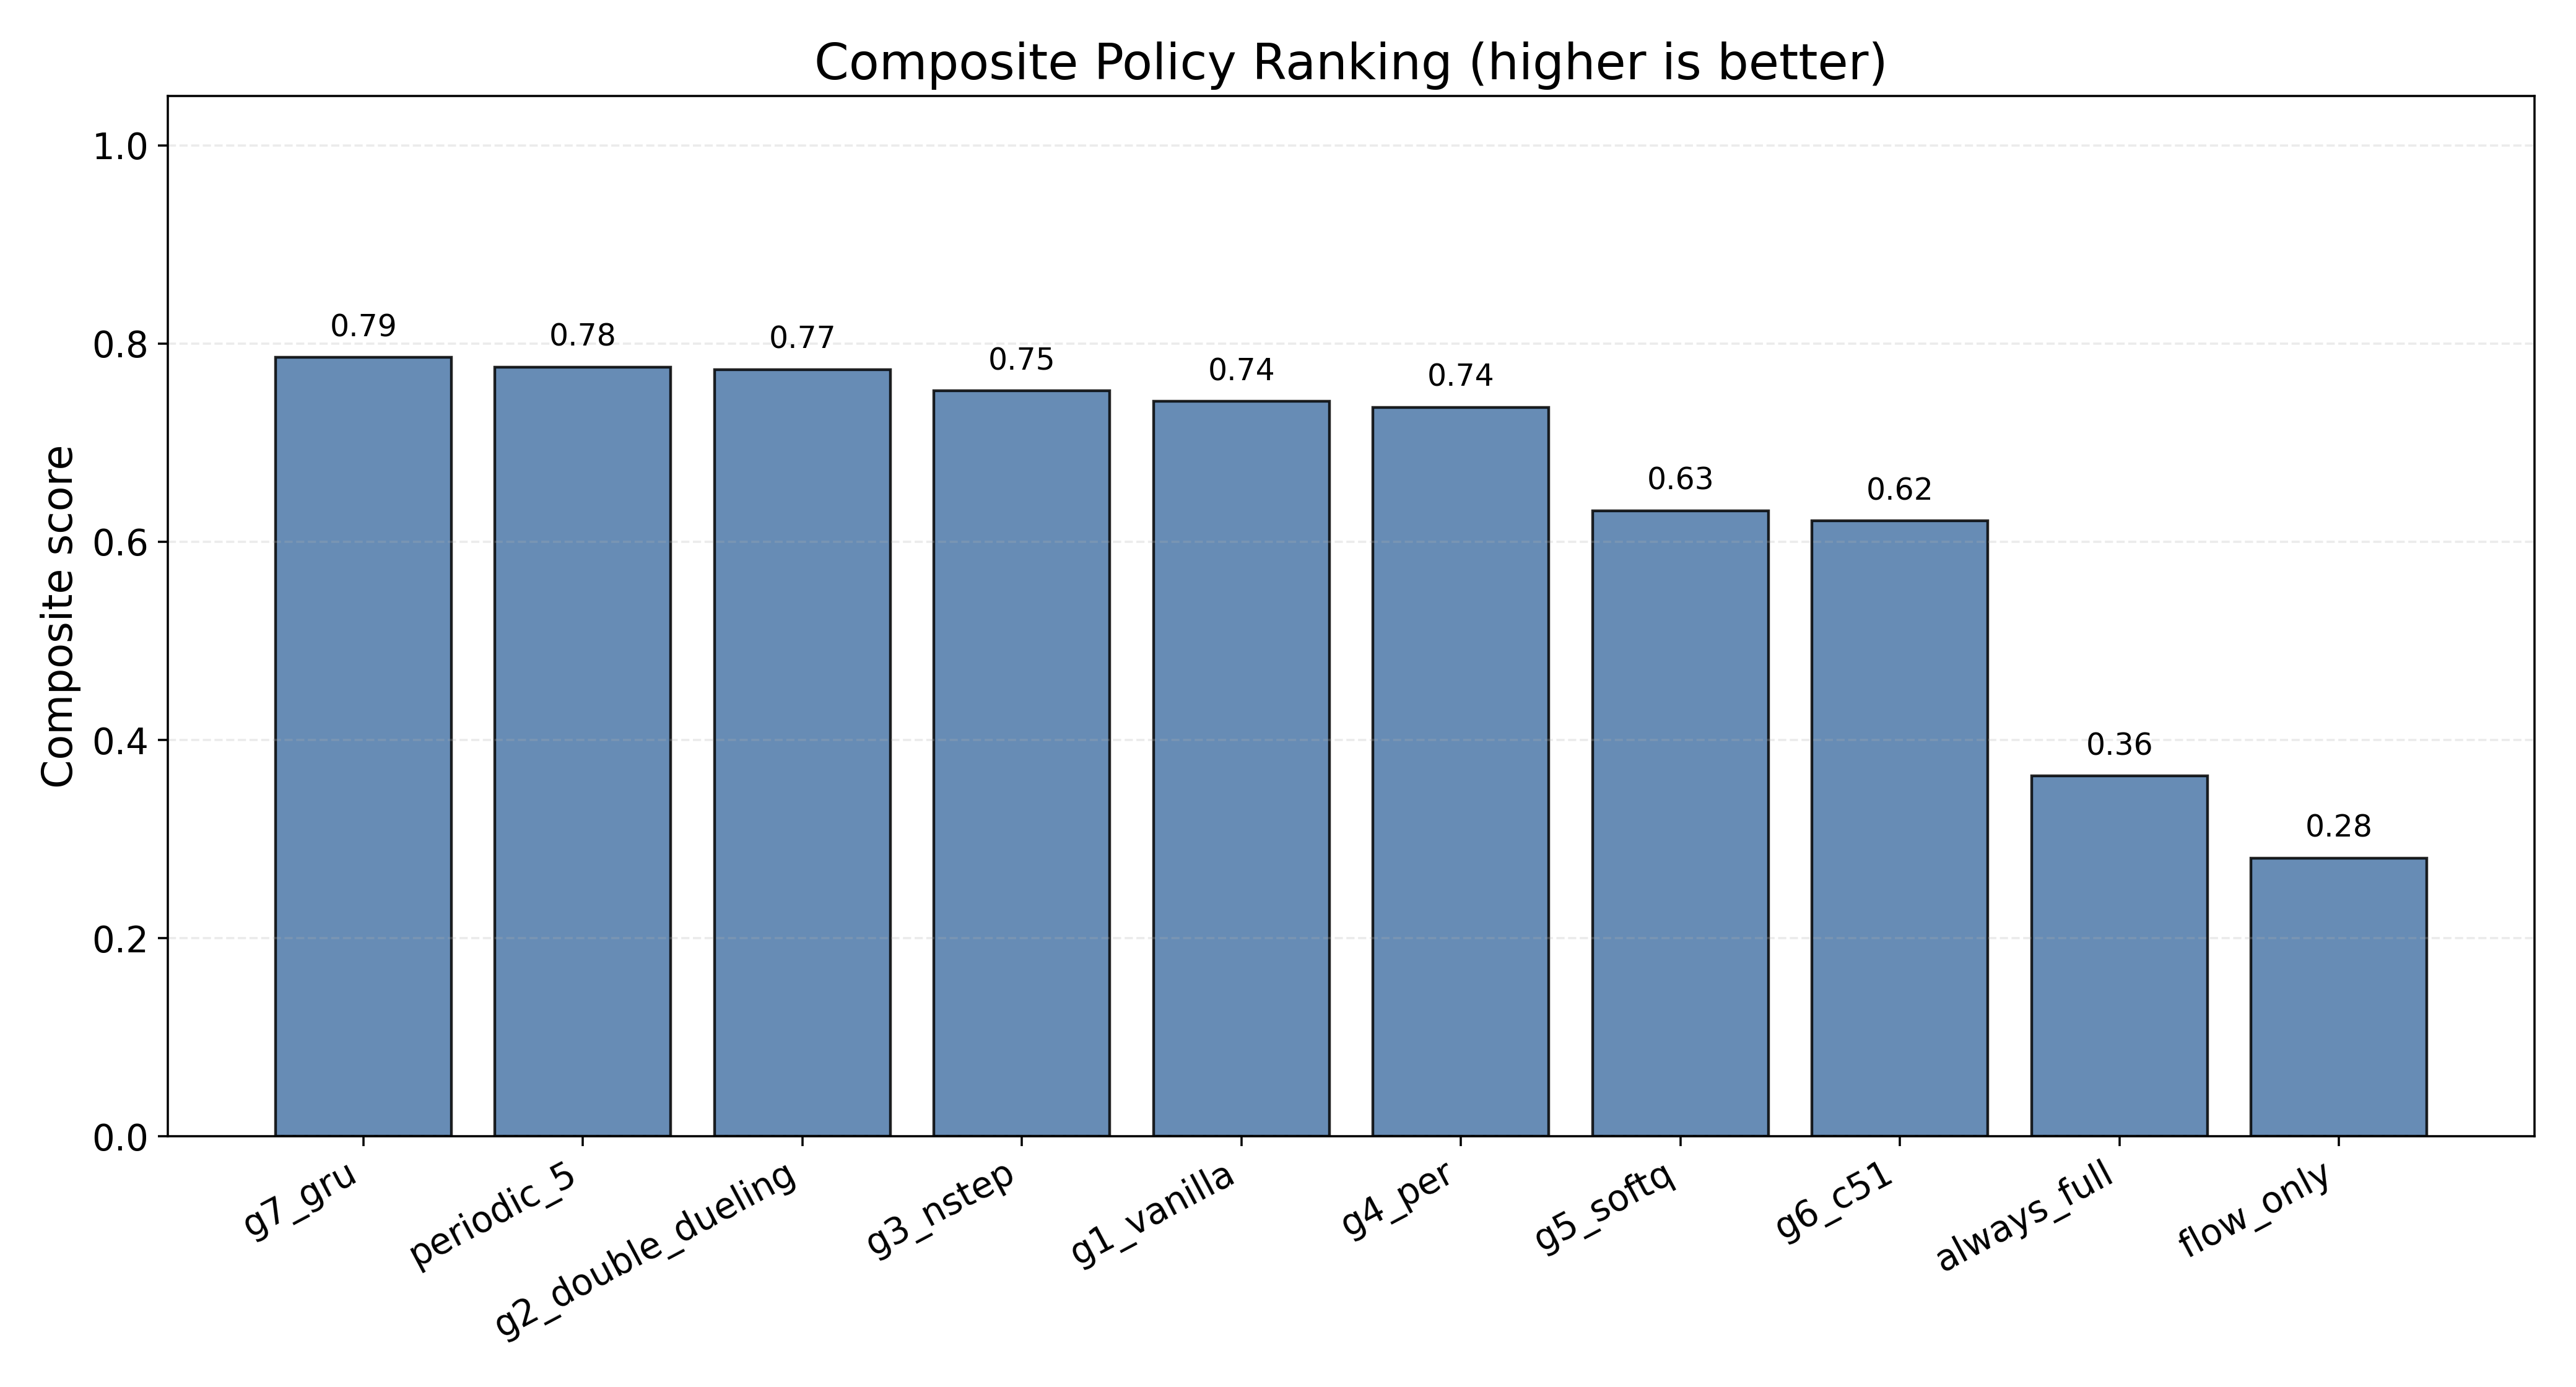
\includegraphics[width=0.96\linewidth]{plots/09_composite_score_ranking_bar.png}
\caption{Composite ranking after per-metric normalization (implicit scalar trade-off); use only after inspecting disaggregated metrics.}
\label{fig:composite_rank}
\end{figure}%
\noindent\textbf{Analysis for Fig.~\ref{fig:composite_rank}.}
The composite plot collapses return, IoU, consistency, and cost into a \emph{single} scalar after per-metric normalization, then ranks policies by that scalar. It is best used as a \textbf{tie-breaker} after understanding Figs.~\ref{fig:return_bar}--\ref{fig:return_cost}: any scalarization hides trade-offs, and the ranking can move if cost is up-weighted relative to IoU (or vice versa).

Read the ordering as ``who is best under the figure's implicit compromise rule,'' not as ground truth. Methods that win only on one axis (e.g., extreme cost reduction) typically fall because the normalization penalizes one-sided specialization. Robust winners should remain near the top if they are strong on at least two axes without catastrophic weakness on a third; if a policy jumps rank relative to Table~\ref{tab:summary_full}, inspect which metric normalization helped or hurt it.

\begin{figure}[H]
\centering
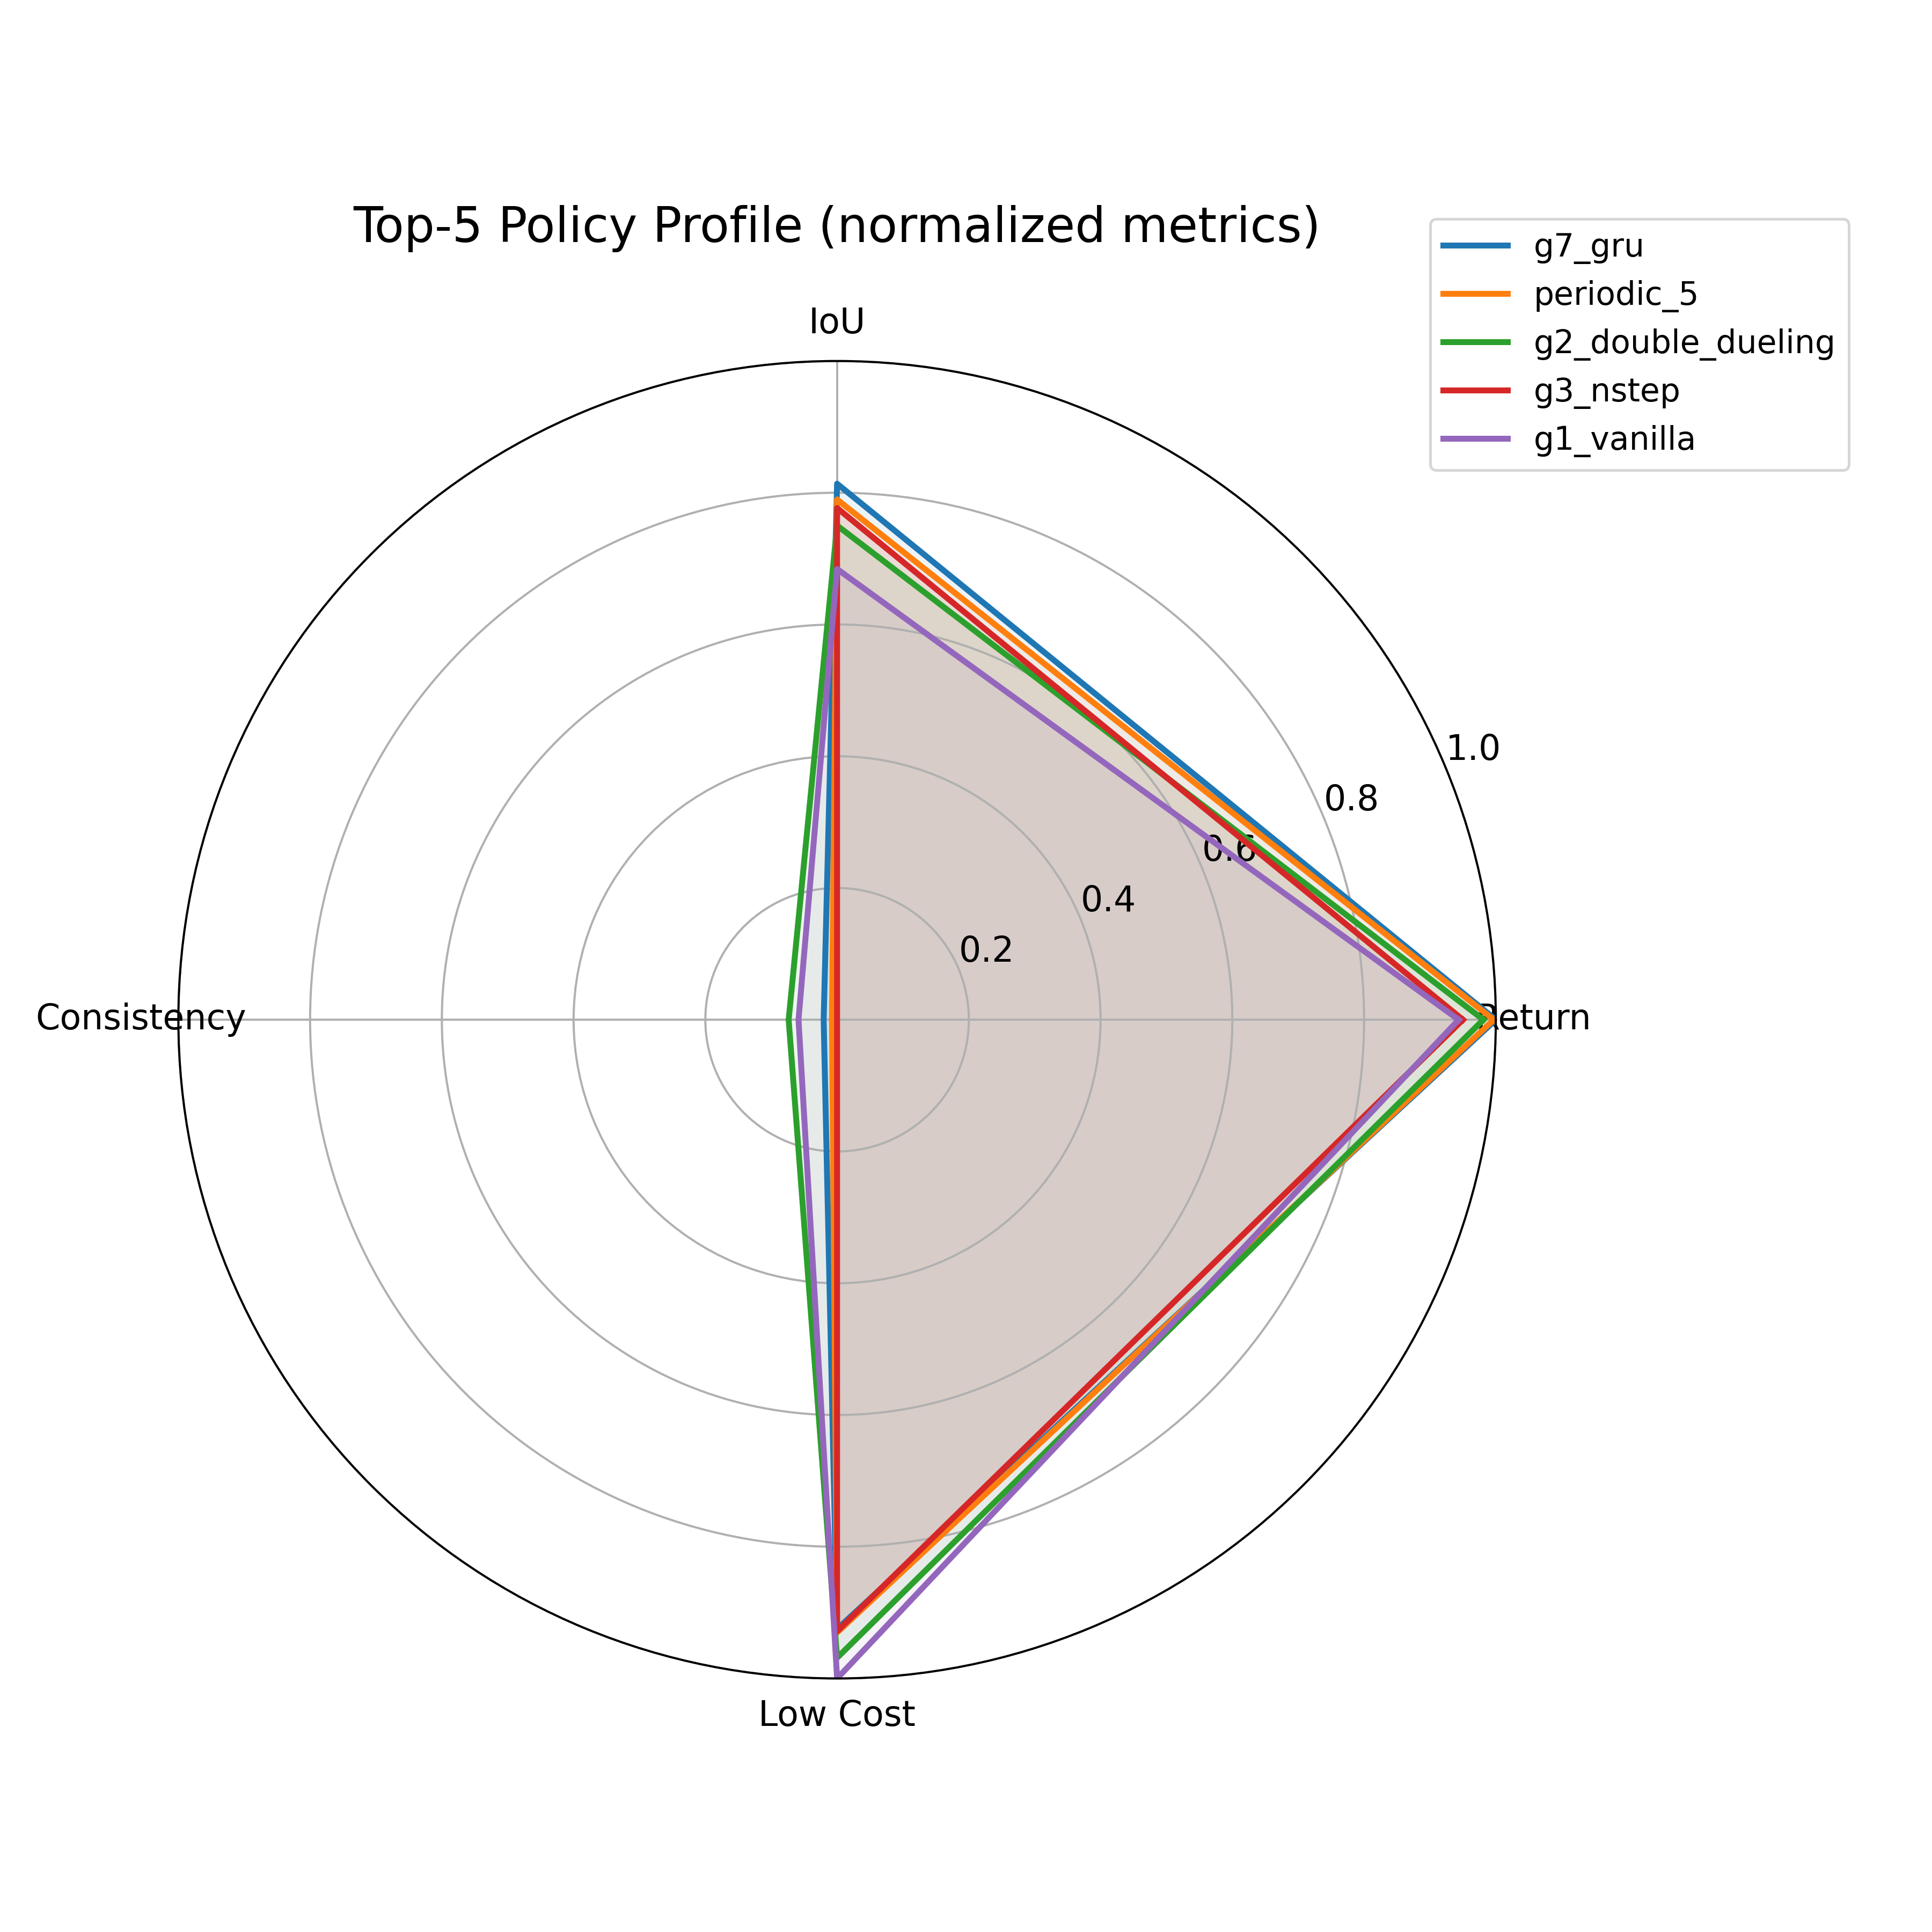
\includegraphics[width=0.96\linewidth]{plots/10_top5_policy_radar.png}
\caption{Top-five policies by composite score: radar axes are normalized metrics for \emph{shape} comparison, not raw units.}
\label{fig:top5_radar}
\end{figure}%
\noindent\textbf{Analysis for Fig.~\ref{fig:top5_radar}.}
The radar chart restricts attention to the top handful of policies by composite score, expanding each axis so shape differences become visible. Each axis is a normalized metric; a balanced polygon means ``no terrible weakness,'' while a spike on one axis and collapse on another reveals specialization.

Use this figure to compare \textbf{profiles}, not raw magnitudes. Two policies with similar return in Fig.~\ref{fig:return_bar} can differ sharply here: one might achieve return via IoU dominance with moderate cost, while another might trade slightly lower IoU for very low cost---the radar makes that shape explicit. For deployment constraints (e.g., ``IoU must stay above $\tau$ while minimizing cost''), look for a polygon whose IoU vertex clears the implicit threshold while the cost vertex is still competitive; if two candidates overlap on IoU but differ on consistency, prefer the smoother profile when downstream modules are noise-sensitive.

\begin{figure}[H]
\centering
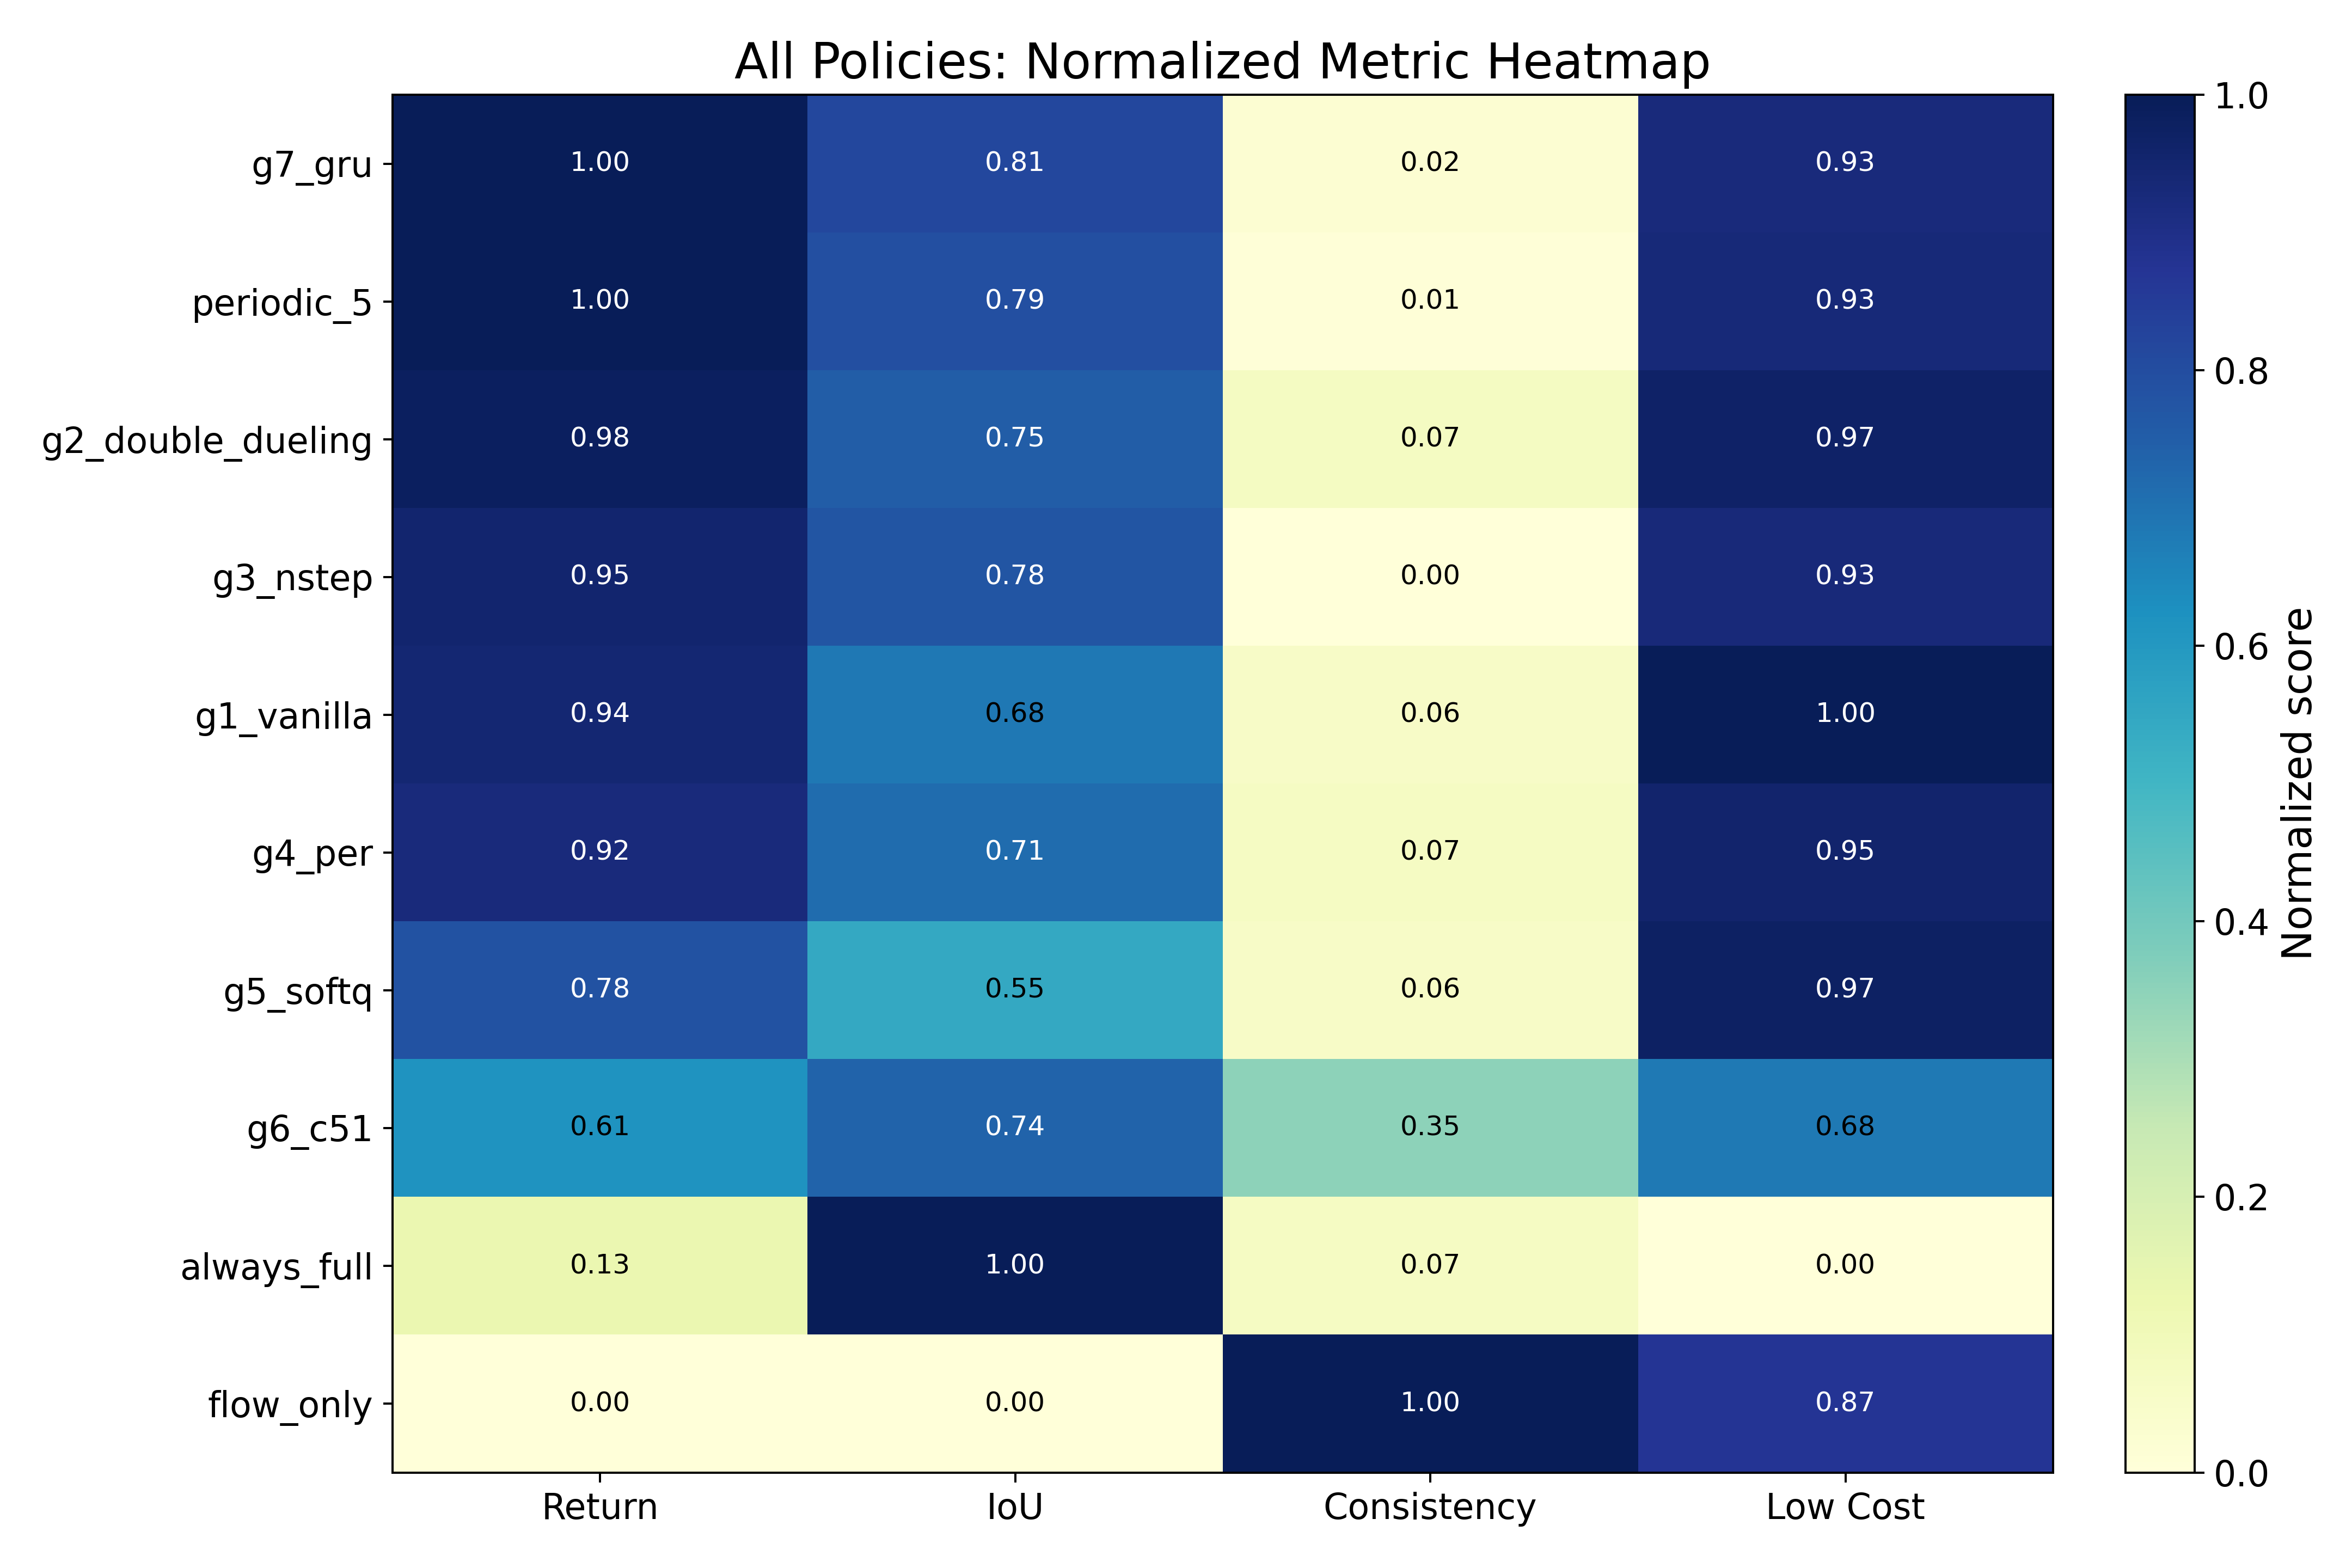
\includegraphics[width=0.96\linewidth]{plots/11_normalized_metric_heatmap_all_policies.png}
\caption{Policy$\times$metric heatmap after normalization: scan rows for balanced strength vs.\ asymmetric weaknesses.}
\label{fig:heatmap_all}
\end{figure}%
\noindent\textbf{Analysis for Fig.~\ref{fig:heatmap_all}.}
Each row is one policy and each column is one metric, after normalization so that colors are comparable across different units. Scan rows for \textbf{uniformly dark ``good'' cells} versus \textbf{stripe patterns} that reveal asymmetry: e.g., strong consistency with weak IoU (smooth wrong track) or strong IoU with weak return (quality exists but reward integration is poor, often due to cost spikes).

The heatmap is especially useful for spotting ``false friends'': policies that look mid-ranked on return alone but have a glaring red cell on cost or IoU that would disqualify them under a stricter constraint. It also makes clear that no policy in this study simultaneously maximizes every column: Always-Full wins IoU but loses cost; Flow-Only loses IoU; some RL variants improve one column at visible expense to another. Model selection should therefore be stated as a \emph{constrained choice} (pick the best row subject to IoU $\ge\tau$ and cost $\le B$), not as picking the single darkest cell in one column.

\subsection{Result interpretation}
The results reveal a stable quality--cost frontier:
\begin{enumerate}[leftmargin=1.4em]
    \item \textbf{Upper-quality anchor:} Always-Full reaches near-perfect IoU at maximal cost.
    \item \textbf{Best learned balance:} G7-GRU attains the top learned IoU and highest return in Table~\ref{tab:summary_full}.
    \item \textbf{Strong heuristic competitor:} Periodic-5 is highly competitive and essential for fair comparative claims.
    \item \textbf{Method sensitivity:} advanced variants are not uniformly superior under this budget (e.g., G6-C51 shows high cost alongside strong consistency in Table~\ref{tab:summary_full}).
\end{enumerate}
These observations are also consistent with the broader message from Rainbow-style ablation results: adding components can help, but gains are context-dependent and may not transfer uniformly across domains without task-specific tuning~\cite{hessel2018rainbow}.

\section{Discussion}

\paragraph{Practical implications.}
The results support treating RL as a \emph{scheduling layer} above a fixed detector stack: the expensive operator remains unchanged, but its invocation frequency is adapted online. In this protocol, G7-GRU and Periodic-5 occupy a similar region of the quality--cost plane (Table~\ref{tab:summary_full} and Figs.~\ref{fig:pareto_iou_cost}--\ref{fig:return_cost}), which is the regime that matters for fixed-camera deployments where ``always on'' full inference is wasteful but blind cost-cutting destroys tracks. The positive takeaway is not that RL always beats every heuristic, but that a learned policy can match a strong periodic schedule while exposing additional algorithmic knobs (backups, replay, recurrence) that the fixed rule does not provide.

\paragraph{What the evidence does (and does not) support.}
All returns and IoU numbers are defined relative to the stated reward and logging pipeline (Sections~\ref{sec:problem} and~\ref{sec:method}). Learned policies therefore optimize \emph{alignment to the offline reference trajectory under the encoded cost model}, not an independent notion of biological or ecological optimality. Claims about ``best'' policies should be read as rankings under these metrics on the evaluated video slice, not as guarantees under camera motion, lighting, or species distribution shifts. That scope statement is important when communicating results to stakeholders who may otherwise over-read a leaderboard table.

\paragraph{Why recurrence and baselines matter here.}
Partial observability is structurally plausible: engineered features compress each frame, and drift can accumulate across frames before it becomes visible in a single vector. A GRU-based value model is a direct response to that mismatch between what the Markov state pretends to summarize and what video actually contains~\cite{hausknecht2015drqn}. At the same time, Periodic-5 shows that a simple open-loop schedule can be surprisingly competitive when the video statistics are benign. Together, these points echo a recurring RL engineering lesson: strong non-learning references are not optional decorations; they define the credibility region in which RL gains are meaningful~\cite{sb3,cleanrldocs}.

\paragraph{Why ``more RL machinery'' is not automatically better.}
Rainbow-style composition suggests that n-step targets, prioritized replay, distributional heads, and soft backups can be complementary~\cite{hessel2018rainbow}, but the same literature also warns that components interact with data volume, reward scale, and optimization noise. The spread among G3--G7 in Table~\ref{tab:summary_full} is consistent with that caution: distributional and backup variants change optimization geometry and can trade cost against stability in ways that only show up when IoU, cost, and consistency are read jointly. This is a reminder to treat algorithm cards as hypotheses to be validated under the target logging protocol, not as monotonic improvements~\cite{bellemare2017distributional,schaul2015per}.

\paragraph{Protocol and metrics as part of the scientific claim.}
Because Gymnasium-style termination semantics and consistent logging change what transitions mean for replay and bootstrapping~\cite{gymapi,gymstep}, Sections~\ref{sec:problem} and~\ref{sec:method} are not ancillary detail: they are part of the claim's meaning. Likewise, tracking-style benchmarks emphasize transparent splits and failure reporting~\cite{lealtaixe2015mot}; at smaller scale, the analogous discipline is to keep $\lambda_{\mathrm{cost}}$, episode caps, and per-episode seeds fixed across policies, which is what enables the Pareto-style reading in Section~\ref{sec:exp_results}.

\paragraph{Deployment-facing risks (even if numbers look good).}
Beyond mean IoU, operators care about tail risk: occasional large drops in quality under rare motion patterns, sensitivity to detector upgrades, and latency variance when \texttt{FULL\_DETECT} is triggered in bursts. The episode boxplots (Fig.~\ref{fig:variability}) and the wide CIs in Table~\ref{tab:ci} are early indicators that deployment decisions should incorporate variance-aware criteria (constraints on worst-episode IoU or cost spikes), not only mean summaries.

\paragraph{Limitations and how to read this section.}
The evaluation uses three episodes per policy; Table~\ref{tab:ci} therefore reports wide normal-theory half-widths rather than tight inference, and no formal significance tests are supplied. The study is also single-video in the headline tables. These constraints do not invalidate the directional patterns, but they do bound the strength of comparative language: the discussion above interprets evidence under a fixed protocol, not a definitive ordering of algorithms for all fish-tracking deployments.

\section{Conclusion}
This report presents an RL-based approach for adaptive compute allocation in fish tracking, formalized as a discrete-action control problem. Across multiple DQN-family variants and non-learning baselines, the experiments consistently show that learned policies can preserve high tracking quality while reducing cost relative to always-full detection.

The strongest empirical outcome under the reported protocol is that the recurrent value-based policy G7-GRU attains the best learned quality--cost trade-off in Table~\ref{tab:summary_full}. The comparison also underscores the need for strong non-learning baselines (Periodic-5) and for protocol-consistent evaluation when interpreting RL gains.

Future work can improve both performance and confidence in several concrete ways. First, expand evaluation breadth (more seeds, more videos, fixed split protocols, tighter intervals with larger $n$, and formal hypothesis tests) to reduce ranking uncertainty. Second, improve learning stability through systematic hyperparameter sweeps (reward scaling, target-update schedule, replay settings, and exploration schedules) and model selection using validation checkpoints rather than always deploying the final \texttt{last.pt} weights. Third, test stronger sequence models (longer context GRU/LSTM or lightweight attention) to better handle partial observability and delayed drift accumulation. Fourth, extend objective design to constraint-aware training (e.g., explicit cost budgets or Lagrangian penalties) so policies are directly optimized for deployment constraints. Finally, improve transfer robustness by testing on different fish videos, camera conditions, and motion regimes, which can reveal whether current gains are general or environment-specific.

\begin{thebibliography}{99}
\bibitem{watkins1992q}
Watkins, C. J. C. H.; and Dayan, P. 1992.
Q-learning.
\textit{Machine Learning}, 8(3--4): 279--292.

\bibitem{tesauro1995td}
Tesauro, G. 1995.
Temporal Difference Learning and TD-Gammon.
\textit{Communications of the ACM}, 38(3): 58--68.

\bibitem{sutton1999pg}
Sutton, R. S.; McAllester, D.; Singh, S.; and Mansour, Y. 1999.
Policy Gradient Methods for Reinforcement Learning with Function Approximation.
\textit{Advances in Neural Information Processing Systems (NeurIPS)}, 12.

\bibitem{mnih2015human}
Mnih, V., et al. 2015.
Human-level control through deep reinforcement learning.
\textit{Nature}, 518(7540): 529--533.

\bibitem{howard2017mobilenets}
Howard, A. G.; Zhu, M.; Chen, B.; Kalenichenko, D.; Wang, W.; Weyand, T.; Andreetto, M.; and Adam, H. 2017.
MobileNets: Efficient Convolutional Neural Networks for Mobile Vision Applications.
\textit{arXiv preprint arXiv:1704.04861}.

\bibitem{vanhasselt2015double}
van Hasselt, H.; Guez, A.; and Silver, D. 2015.
Deep Reinforcement Learning with Double Q-learning.
\textit{Proceedings of the AAAI Conference on Artificial Intelligence}, 30(1).

\bibitem{schaul2015per}
Schaul, T.; Quan, J.; Antonoglou, I.; and Silver, D. 2016.
Prioritized Experience Replay.
In \textit{Proceedings of the International Conference on Learning Representations (ICLR)}.

\bibitem{wang2016dueling}
Wang, Z.; Schaul, T.; Hessel, M.; van Hasselt, H.; Lanctot, M.; and de Freitas, N. 2016.
Dueling Network Architectures for Deep Reinforcement Learning.
In \textit{Proceedings of the International Conference on Machine Learning (ICML)}, 1995--2003.

\bibitem{hessel2018rainbow}
Hessel, M.; Modayil, J.; van Hasselt, H.; Schaul, T.; Ostrovski, G.; Dabney, W.; Horgan, D.; Piot, B.; Azar, M.; and Silver, D. 2018.
Rainbow: Combining Improvements in Deep Reinforcement Learning.
In \textit{Proceedings of the AAAI Conference on Artificial Intelligence}, 32(1).

\bibitem{bellemare2017distributional}
Bellemare, M. G.; Dabney, W.; and Munos, R. 2017.
A Distributional Perspective on Reinforcement Learning.
In \textit{Proceedings of the International Conference on Machine Learning (ICML)}, 449--458.

\bibitem{hausknecht2015drqn}
Hausknecht, M.; and Stone, P. 2015.
Deep Recurrent Q-Learning for Partially Observable MDPs.
In \textit{Proceedings of the AAAI Fall Symposium on Sequential Decision Making for Intelligent Agents}.

\bibitem{lealtaixe2015mot}
Leal-Taix\'e, L.; Milan, A.; Reid, I.; Roth, S.; and Schindler, K. 2015.
MOTChallenge 2015: Towards a Benchmark for Multi-Target Tracking.
\textit{arXiv:1504.01942}.

\bibitem{gymapi}
Farama Foundation.
Gymnasium Env API.
\url{https://gymnasium.farama.org/api/env/}.

\bibitem{gymstep}
Farama Foundation.
Gymnasium Terminated/Truncated Step API rationale.
\url{https://farama.org/Gymnasium-Terminated-Truncated-Step-API}.

\bibitem{sb3}
Stable-Baselines3 Documentation.
\url{https://stable-baselines3.readthedocs.io/en/master/}.

\bibitem{cleanrldocs}
CleanRL Documentation.
\url{https://docs.cleanrl.dev/}.
\end{thebibliography}

\end{document}
